%-------------------------------------------------------------------------------
%                      Template Naskah Skripsi
%               	Berdasarkan format JTETI FT UGM
% 						(c) @gunturdputra 2014
%-------------------------------------------------------------------------------

%Template pembuatan naskah skripsi.
\documentclass{jtetiskripsi}

%Untuk prefiks pada daftar gambar dan tabel
\usepackage[titles]{tocloft}
\renewcommand\cftfigpresnum{Gambar\  }
\renewcommand\cfttabpresnum{Tabel\   }

%Untuk hyperlink dan table of content
\usepackage[hidelinks]{hyperref}
\newlength{\mylenf}
\settowidth{\mylenf}{\cftfigpresnum}
\setlength{\cftfignumwidth}{\dimexpr\mylenf+2em}
\setlength{\cfttabnumwidth}{\dimexpr\mylenf+2em}

%Untuk Bold Face pada Keterangan Gambar
\usepackage[labelfont=bf]{caption}

%Untuk caption dan subcaption
\usepackage{caption}
\usepackage{subcaption}

%pdf
\usepackage{pdfpages}

%table
\usepackage{graphics}

\usepackage{wrapfig}


%equation
\usepackage{amsmath}

%hypenat
%\usepackage[none]{hyphenat}/

%bibliography
\usepackage{natbib}

%-----------------------------------------------------------------
%Disini awal masukan untuk data proposal skripsi
%-----------------------------------------------------------------
\titleind{Deteksi Keliling Luka menggunakan \break \emph{Parametric Active Contour}}

\fullname{Muhamad Rizki}

\idnum{3145160661}

%\approvaldate{-}
\approvaldate{-}

\degree{Sarjana Ilmu Komputer}

\yearsubmit{2020}

\program{Ilmu Komputer}

\dept{Ilmu Komputer}

\firstsupervisor{Med Irzal, M. Kom.}
\firstnip{197706152003121001}

\secondsupervisor{Muhammad Eka Suryana, M. Kom.}
\secondnip{198512232012121002}

%hypenation


%-----------------------------------------------------------------
%Disini akhir masukan untuk data proposal skripsi
%-----------------------------------------------------------------

\tolerance=1
\emergencystretch=\maxdimen
\hyphenpenalty=10000
\hbadness=10000

\begin{document}
\cover
%-----------------------------------------------------------------

%-----------------------------------------------------------------
%Disini akhir masukan untuk muka skripsi
%-----------------------------------------------------------------

\tableofcontents 
\addcontentsline{toc}{chapter}{DAFTAR ISI}
\listoffigures
\addcontentsline{toc}{chapter}{DAFTAR GAMBAR}
\listoftables
\addcontentsline{toc}{chapter}{DAFTAR TABEL}

\begin{counterpage}
\end{counterpage}
%Disini awal masukan untuk Bab
%-----------------------------------------------------------------
%!TEX root = ./template-skripsi.tex
%-------------------------------------------------------------------------------
% 								BAB I
% 							LATAR BELAKANG
%-------------------------------------------------------------------------------

\chapter{PENDAHULUAN}
\section{Latar Belakang Masalah}

Luka kronis adalah masalah kritis dalam kesehatan. Di Amerika Serikat, sekitar 6,5 juta orang menderita luka kronis dan biaya perawatan luka kronis menghabiskan sekitar \$20 miliar per tahun. Bahkan di negara maju, sekitar 1-2\% dari seluruh populasi terkena luka kronis selama hidup mereka. \citep{Biswas2018superpixel:1}. Luka kronis berdampak terhadap finansial dan penurunan kualitas hidup pasien. Kerusakan fisik, sosial, dan emosional seperti penurunan mobilitas, rasa sakit, ketidaknyamanan, membatasi kinerja aktivitas sehari-hari. Isolasi sosial, frustasi, dan reaksi psikologis lainnya yang menimbulkan dampak pada kehidupan pasien. \citep{NaiaraVogt2020quality:2}. Di Indonesia sendiri pengidap luka kronis berjumlah sekitar 24\% dari 8,6\% total populasi terhadap kasus diabetes. \citep{Safitri2022hubungan:3}. 

Pada penelitian sebelumnya yang dilakukan oleh Salsa yang berjudul "Rancang Bangun Aplikasi dan \emph{Web Service} Pengkajian Luka Kronis Khusus Modul Pengolahan Citra Berbasis Android". Salsa melakukan wawancara dengan Ratna Aryani, M.Kep., Dosen Politeknik Negeri Jakarta I, diperoleh bahwa saat melakukan penggantian balutan luka dan pengecekan awal kondisi luka dilakukan pengkajian luka. Berikut  langkah-langkah pengkajian luka diawali dengan balutan luka dibuka, lalu luka dicuci, dan diakhiri dengan proses pengkajian luka. Instrumen yang dipilih saat melakukan pengkajian luka ialah Bates-Jensen \emph{Wound Assesment Tools} (BWAT). Pada BWAT ada 13 kategori penilaian yakni beberapa di antaranya  tepi luka, ukuran luka, epitalisasi dan jumlah eksudat (cairan tubuh yang keluar dari jaringan selama peradangan). Saat ini data pengkajian luka masih dilakukan secara tradisional dicatat dalam arsip atau catatan kertas, maka dari itu salsa mengusulkan untuk mendigitalisasi pencatatan data luka yang sudah dikaji. \citep{Rahmadati2023rancang:4}.

Penelitian lain yang terkait juga dilakukan oleh Ardiansyah, menjelaskan bahwa Rumah Sakit Umum Kambang Jambi masih memakai cara tradisional dalam pelayanannya seperti mendapatkan nomor antrian berobat, informasi mengenai jadwal dokter dan jumlah seluruh pasien. Hal ini menyebabkan pemanfaatan informasi menjadi kurang maksimal, berjalan kurang efektif dan lama dalam prosesnya. Dengan adanya permasalahan yang terjadi ardiansyah dan kawannya menyimpulkan bahwa dibutuhkannya Sistem Informasi Manajemen Rumah Sakit Berbasis \emph{Website} untuk menyelesaikan permasalahan yang ada. Sehingga meminimalkan kekurangan dan ketidak efektifan dalam pelayanan. \citep{Ardiansyah2021analisis:10}.

Dalam jurnal berjudul "Sistem Informasi Rekam Medis Pada Rumah Sakit Umum Daerah (RSUD) Pacitan Berbasis \emph{Web Base}" oleh Gunawan Susanto. Pencatatan riwayat dan data rekam medis kesehatan milik pasien merupakan hal yang krusial dalam dunia medis karena data tersebut digunakan untuk pemeriksaan pasien selanjutnya. Sistem pencatatan yang dipakai memiliki kelemahan. Hal ini dikarenakan data rekam medis pasien hanya disimpan secara lokal di tempat pasien diperiksa dan dirawat serta pertukaran data langsung antara divisi medis tidak diperbolehkan. Maka dari itu dilakukan pengembangan sistem informasi rekam medis yang memiliki tujuan untuk menyelesaikan kelemahan yang dimiliki oleh sistem pencatatan rekam medis pasien yang sebelumnya, yaitu alternatif teknologi yang dapat diterapkan di masa yang akan datang untuk pencatatan dan penyampaian data rekam medis. \citep{Gunawan2011sistem:11}.

Pada penelitian yang dilaksanakan oleh Inah Carminah yang berjudul "Aplikasi Monitoring Perawatan Luka Diabetes Melitus Berbasis \emph{Website}". Proses pelayanan yang masih menggunakan \emph{paper base system} memiliki risiko kerusakan atau kehilangan data rekam medis pasien. Selain itu membuat perawat kewalahan ketika mencari data rekam medis pasien secara satu-persatu ketika dibutuhkan ketika pasien datang untuk berobat kembali. Berangkat dari permasalahan di atas memotivasi instansi untuk membuat apikasi dengan tujuan untuk meningkatkan kualitas pelayanan pasien saat berobat. \citep{Carminah2021aplikasi:12}.

%
Didalam buku berjudul “Rancang Bangun Aplikasi \emph{Mobile} Android Sebagai Alat Deteksi Warna Dasar Luka Dalam Membantu Proses Pengkajian Luka Kronis Dengan Nekrosis”, Tehnik pengkajian luka berdasarkan warna luka yang umum digunakan salah satunya The RYB (\emph{Red-Yellow-Black}) \emph{wound classification system}. Metode ini digunakan dengan mengandalkan subyektifitas dari perawat luka. Hasil penelitian pada buku ini menunjukkan bahwa perawat mampu mengetahui perbedaan warna luka secara otomatis yang membantu proses pengkajian luka kronis dengan nekrosis. \citep{Aryani2018rancang:6}. Ia juga meneliti dan menemukan bahwa perban basah membantu mempercepat proses penyembuhan luka. Perawat harus mempertimbangkan untuk menggunakan balutan basah daripada perawatan standar untuk meningkatkan penyembuhan. Namun, perawat harus melindungi luka dari kelembapan yang berlebihan karena dapat merusak kulit di sekitar luka atau di dalam luka. \citep{Aryani2016accelerating:7}.

%
Pada payung penelitian \emph{medical imaging} yang sama dengan peneliti juga sudah pernah dilakukan penelitian mengenai Pengaruh Penggunaan \emph{Color Model} LAB dalam Kalibrasi Warna Luka Menggunakan Metode Segmentasi K-\emph{Means} dan \emph{Mean Shift} oleh rekan sesama peneliti. \citep{Khairunnisa2021pengaruh:8}. Dan Muhamad rizki juga melakukan penelitian deteksi tepi luka menggunakan metode \emph{Active Contour} yang ditambah interpolasi. \citep{Rizki2022deteksi:9}. Kedua penelitian tersebut merupakan penelitian berdasarkan dua kategori pengkajian luka yaitu warna luka dan tepi luka, algoritma yang dikembangkan pada penelitian tersebut direncanakan akan terintegrasi dalam satu ekosistem aplikasi, yakni sistem informasi keperawatan luka. Dimana pada penelitian Salsa Rahmadati melakukan perancangan aplikasi pengkajian luka kronis berbasis Android sesuai modul \emph{image processing}. \citep{Rahmadati2023rancang:4}. 

%
Berdasarkan hal di atas, penulis tertarik untuk melakukan penelitian yang bertujuan untuk membuat sistem informasi keperawatan luka dengan dasar pengembangan menggunakan data paparan presentasi bersama ibu Irma Puspita Arisanti selaku pemilik klinik \emph{moist care} dan sesuai dengan proposal PKM-PI dengan judul "Pengembangan Pelayanan Sistem Informasi Klinik Serta Fitur Keperawatan Luka Pada Aplikasi Untuk Mendukung Integrasi Data Kesehatan Dan Ketahanan Nasional Bidang Kesehatan" yang dibuat oleh Hafiz dan tim. Melanjutkan penelitian sebelumnya yang dilakukan oleh Salsa, dimana pengkajian luka masih dilakukan dengan cara manual atau arsip kertas sehingga Salsa membuat aplikasi untuk mengarsipkan data secara digital dan peneliti mengembangkan \emph{web} aplikasi yang berkaitan dengan aplikasi sebelumnya untuk dapat diakses datanya oleh klinik dengan maksud seluruh staff klinik yang berkepentingan dapat dengan mudah mengaksesnya.
 
Sistem Informasi tersebut diharapakan dapat menambah opsi pendaftaran berobat secara \emph{online} selain daripada pendaftaran secara \emph{offline}, membantu pengelolaan antrian, membantu integrasi data pasien dan perawat secara digital, manajemen invetaris, beserta verifikasi dan validasi biaya tagihan sehingga dapat mempermudah pelayanan.  

\section{Rumusan Masalah}
Berdasarkan uraian pada latar belakang yang diutarakan di atas, maka perumusan masalah pada penelitian ini adalah bagaimana membuat rancang bangun sistem informasi keperawatan luka?

\section{Pembatasan Masalah}
Batasan masalah dalam penelitian ini adalah:

\begin{enumerate}
	\item Sistem informasi keperawatan luka dibuat dengan dasar instrumen pengkajian Bates-Jensen \emph{Wound Assessment Tool} (BWAT).
	
	\item \emph{User} aplikasi sistem informasi keperawatan luka adalah perawat dan admin klinik.
	
	\item Sistem informasi keperawatan luka dibuat berbasis \emph{Website}
	
	\item Sistem informasi keperawatan luka dibuat berdasarkan paparan presentasi bersama pemilik klinik \emph{Moist Care} yaitu ibu Irma Puspita Arisanti.
	
	\item Model pengembangan yang digunakan untuk mengembangkan sistem informasi keperawatan luka adalah \emph{scrum}.
	
	\item Fitur-fitur yang diimplementasi pada sistem informasi keperawatan luka, diantaranya adalah pembuatan akun pasien, \emph{dashboard} klinik, pemeriksaan kesehatan dan sebagian proses pengobatan luka (\emph{view} dan \emph{web service} inventaris dan layanan).
	
\end{enumerate}

\section{Tujuan Penelitian}
Penelitian ini bertujuan untuk membuat rancang bangun sistem informasi keperawatan luka di klinik \emph{Moist Care}.

\section{Manfaat Penelitian}
\begin{enumerate}
	\item Bagi penulis
	
	Penelitian yang dilakukan merupakan media penerapan dari berbagai ilmu pengetahuan, khususnya dalam perancangan sistem informasi keperawatan luka pada klinik \emph{Moist Care}.
	
	\item Bagi Program Studi Ilmu Komputer
	
	Penelitian ini dapat menjadi pintu gerbang untuk penelitian selanjutnya di masa depan.
	
	\item Bagi Universitas Negeri Jakarta
	
	Menjadi evaluasi akademik program studi Ilmu Komputer dalam penulisan skripsi sehingga dapat meningkatkan kualitas pendidikan program studi Ilmu Komputer di Universitas Negeri Jakarta.
	
\end{enumerate}

% Baris ini digunakan untuk membantu dalam melakukan sitasi
% Karena diapit dengan comment, maka baris ini akan diabaikan
% oleh compiler LaTeX.
\begin{comment}
\bibliography{daftar-pustaka}
\end{comment}

%!TEX root = ./template-skripsi.tex
%-------------------------------------------------------------------------------
%                            BAB II
%               KAJIAN TEORI
%-------------------------------------------------------------------------------

\chapter{KAJIAN PUSTAKA}

\section{Sistem Informasi}

Sistem informasi tersusun dari dua kata yaitu sistem dan informasi. Menurut Jerry FitzGerald, Sistem adalah suatu jaringan kerja dari prosedur-prosedur yang saling berhubungan berkumpul bersama-sama untuk melakukan suatu kegiatan atau menyelesaikan suatu sasaran tertentu. Suatu sistem terdiri dari sejumlah komponen yang saling berinteraksi, bekerja sama membentuk satu kesatuan. Komponen-komponen sistem dapat berupa suatu subsistem atau bagian-bagian dari sistem. Setiap sistem tidak perduli betapapun kecilnya, selalu mengandung komponen-komponen atau subsistem-subsistem. Setiap subsistem mempunyai sifat-sifat dari sistem untuk menjalankan suatu fungsi tertentu dan mempengaruhi proses sistem secara keseluruhan. \citep{FitzGerald1981Fundamental:14}

Informasi adalah data yang telah diproses menjadi bentuk yang memiliki arti bagi penerima dan dapat berupa fakta, suatu nilai yang bermanfaat. Jadi ada suatu proses transformasi data menjadi suatu informasi yaitu \emph{input}, proses dan \emph{output}. Menurut Robert A. Leitch, Sistem informasi adalah suatu sistem di dalam suatu organisasi yang mempertemukan kebutuhan pengolahan transaksi harian, mendukung operasi, bersifat manajerial dan kegiatan strategi dari suatu organisasi dan menyediakan pihak luar tertentu dengan laporan-laporan yang diperlukan. \citep{Robert2001Sistem:15}      

\section{Unified Modeling Language (UML)}

Subbab ini ditulis berdasarkan \citep{Suendri2019metode:13}. \emph{Unified Modeling Language} (UML) adalah sebuah bahasa yang berdasarkan grafik atau gambar dalam memvisualisasi, menspesifikasikan, membangun, dan pendokumentasian dari sebuah sistem pengembangan \emph{software} berbasis OO (\emph{Object-Oriented}). Siti Fatima mengatakan UML memberikan standar penulisan dalam sebuah sistem \emph{blueprint} yang meliputi konsep bisnis proses, penulisan kelas-kelas yang spesifik dalam bahasa program, skema database, dan komponen-komponen yang dibutuhkan dalam sistem \emph{sofware} \cite{Fatima2013Perangcangan:14}. 
Diagram \emph{Unified Modelling Language} (UML) antara lain sebagai berikut :

\subsection{\emph{Use Case Diagram}}
\emph{Use case} menggambarkan \emph{external view} dari sistem yang akan kita buat modelnya. Model \emph{use case} dapat diartikan sebagai diagram \emph{use case}, tetapi diagram ini tidak sama dengan model sebab model memiliki cakupan yang lebih luas dari diagram. \emph{Use case} harus sanggup dalam menggambarkan susuan atau urutan aktor yang menghasilkan nilai terukur. \citep{Widodo2011Menggunakan}

\subsection{\emph{Class Diagram}}
Kelas merupakan suatu set objek dengan atribut dan perilaku yang sama. Kelas dapat disebut juga sebagai kelas objek. \citep{Whitten2004Metode}

Kelas memiliki tiga area pokok yaitu :

\begin{enumerate}
	\item Nama, kelas haruslah mempunyai sebuah nama.
	
	\item Atribut, merupakan kelengkapan yang melekat pada kelas. Suatu kelas memiliki nilai yang hanya bisa diproses sebatas pada atribut yang dimiliki.
	
	\item Operasi, merupakan proses yang dilakukan oleh sebuah kelas kepada kelas itu sendiri ataupun kelas lainnya.
\end{enumerate}

\subsection{\emph{Activity Diagram}}
Diagram \emph{activity} menunjukkan aktivitas sistem yang berbentuk kumpulan dari aksi-aksi, bagaimana masing-masing aksi tersebut dimilai, keputusan yang mungkin terjadi hingga berakhirnya aksi. Selain itu, \emph{activity diagram} dapat menggambarkan lebih dari satu prses aksi dalam waktu yang bersamaan. “\emph{Activity diagram } adalah aktifitas-aktifitas, objek, \emph{state}, \emph{transisi state} dan \emph{event}. Dengan kata lain kegiatan diagram alur kerja menggambarkan perilaku sistem untuk aktivitas”. \citep{Haviluddin2011Memahami} 

\subsection{\emph{Sequence Diagram}}
“Secara mudahnya \emph{sequence diagram} adalah gambaran tahap demi tahap, termasuk kronologi (urutan) perubahan secara logis yang seharusnya dilakukan untuk menghasilkan sesuatu sesuai dengan \emph{use case diagram}.”
\citep{Haviluddin2011Memahami}

\section{Pengantar \emph{Flask}}
\emph{Flask} merupakan \emph{web framework} yang memiliki dasar bahasa pemprograman \emph{python}. \emph{Web framework} adalah koleksi dari modul-modul dan \emph{packages} yang membuat pengembang dapat membuat aplikasi \emph{web} atau \emph{web service} tanpa harus memikirkan detail-detail dasar seperti protokol, soket, atau manajemen proses.

\emph{Core} yang dimiliki \emph{flask} tergolong sederhana dan bersifat ringan, selain itu \emph{flask} juga bersifat \emph{simplicity} dan \emph{flexibility} sehingga pengembangan dapat menyesuaikan dengan kebutuhan oleh penambahan ekstensi yang ada. Ekstensi yang dimiliki \emph{flask} salah satunya adalah \emph{blueprint}. \emph{Blueprint} memiliki fungsi untuk mempermudah dalam pembuatan pengaturan minimal RESTful APIs. RESTful APIs merupakan layanan atau metode yang berfungsi untuk mentransimisikan data dengan menggunakan protokol HTTP.

\emph{Routing} pada \emph{flask} diartikan sebagai bantuan ekstensi \emph{blueprint} yang mempermudah akses kepada beberapa metode \emph{Hypertext Transfer Protocol}(HTTP) hanya dengan mendefinisikan metode yang digunakan pada \emph{routing} yang akan digunakan. Metode permintaan HTTP yang bisa gunakan antara lain sebagai berikut:

\begin{table}[H]
	\centering
	\caption{Fungsi-fungsi Metode HTTP}
	\label{tabel_input}
	\begin{tabular}{|m{3cm}|m{9cm}|}
		\hline
		\textbf{Metode HTTP} & \textbf{Fungsi}\\
		\hline
		
		GET &
		\setstretch{1}
		Menerima informasi dari server yang diberikan menggunakan 
		URI yang spesifik. Permintaan menggunakan metode \emph{GET} hanya menerima data tanpa adanya efek perubahan pada data.\\
		\hline
		
		POST &
		\setstretch{1}
		Mengirimkan data ke \emph{server} seperti unggahan \emph{file}, informasi pelanggan dan lain-lain menggunakan \emph{form} HTML.\\
		\hline
		
		HEAD &
		\setstretch{1}
		Sama seperti metode \emph{GET}, namun hanya memberikan data status dan seksi header saja.\\
		\hline
		
		PUT &
		\setstretch{1}
		Mengganti semua representasi dari target \emph{resource} dengan konten yang diunggah.\\
		\hline
		
		DELETE &
		\setstretch{1}
		Menghapus semua representasi dari target yang didefinisikan pada URI.\\
		\hline
		
	\end{tabular}
\end{table}

\begin{figure}[H]
	\centering
	\includegraphics[width=12cm]{gambar/flask1.png}
	\caption{Contoh registrasi Blueprint pada dokumen “auth.py”. \\ Sumber: https://flask.palletsprojects.com/en/2.1.x/tutorial/views/}
	\label{Gambar:registrasi blueprint}
\end{figure}

\textbf{Gambar 2.1} berisi \emph{code} pada halaman sebelumnya berfungsi untuk menterjemahkan penggunaan ekstensi \emph{blueprint} pada suatu dokumen bernama ‘\emph{auth}’. Agar \emph{routing} dapat berjalan maka harus di registrasikan pada dokumen init.py yang merupakan tempat \emph{flask} akan berjalan.

\begin{figure}[H]
	\centering
	\includegraphics[width=8cm]{gambar/flask2.png}
	\caption{Dokumen \_\_init\_\_.py. \\ Sumber: https://flask.palletsprojects.com/en/2.1.x/tutorial/views/}
	\label{Gambar:registrasi blueprint}
\end{figure}

\textbf{Gambar 2.3} merupakan contoh dari pembuatan \emph{routing login} dengan URL \emph{routing} “\emph{/login}” yang mendefinisikan metode \emph{GET} dan \emph{POST}. Saat proses \emph{log in} sukses maka akan diarahkan ke URL “\emph{login}.html”.

\begin{figure}[H]
	\centering
	\includegraphics[width=12cm]{gambar/flask3.png}
	\caption{Contoh pembuatan \emph{routing} dengan \emph{Blueprint}. \\ Sumber: https://flask.palletsprojects.com/en/2.1.x/tutorial/views/}
	\label{Gambar:registrasi blueprint}
\end{figure}

\section{MongoDB}

MongoDB adalah basis data yang menggunakan konsep \emph{Not Only} SQL (NoSQL) yang menyimpan data berorientasikan dokumen. NoSQL tidak memiliki sistem tabular dan mempunyai perbedaan penyimpanan dari tabel relasional. \emph{Database} dengan konsep NoSQL memberikan pengembang fleksibilitas untuk menyimpan struktur data dalam jumlah besar.

Kunci perbedaan NoSQL dan \emph{Relational Database Management System} (RDBMS) ialah bagaimana sebuah data dimodelkan pada \emph{database}. RDBMS menggunakan pemodelan yang masih menggunakan tabel berstruktur dengan setiap kolom baris bersifat tetap antara satu dengan lainnya, sedangkan pemodelan data pada NoSQL, khususnya pada MongoDB, menggunakan dokumen dimana setiap barisnya mempunyai kolom yang dapat berbeda dengan baris yang lain. berikut merupakan contoh perbedaan basis data menggunakan konsep RDBMS dan NoSQL dapat dilihat pada \textbf{Gambar 2.4} (Pemodelan RDBMS) dan \textbf{Gambar 2.5} (Permodelan NoSQL).

\begin{figure}[H]
	\centering
	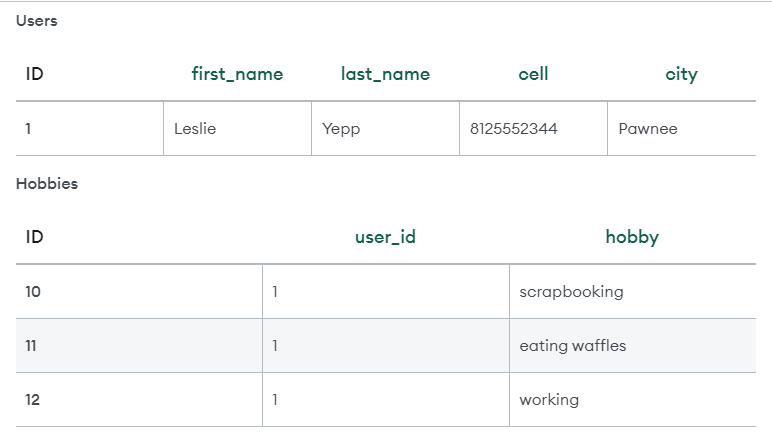
\includegraphics[width=12cm]{gambar/mongoDB1.png}
	\caption{Pemodelan RDBMS. \\ Sumber: https://www.mongodb.com/nosql-explained/}
	\label{Gambar:registrasi blueprint}
\end{figure}

\begin{figure}[H]
	\centering
	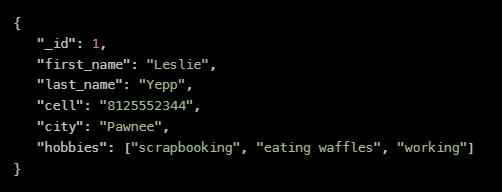
\includegraphics[width=12cm]{gambar/mongoDB2.png}
	\caption{Pemodelan NoSQL. \\ Sumber: https://www.mongodb.com/nosql-explained/}
	\label{Gambar:registrasi blueprint}
\end{figure}

Pada \textbf{Gambar 2.4} pada halaman sebelumnya, digunakan untuk menyimpan data \emph{user} dan data \emph{hobbies} dibutuhkan dua tabel terpisah dimana hal ini tidak dibutuhkan pada pemodelan NoSQL (\textbf{Gambar 2.5}) yang dapat menggabungkan dua data \emph{user} dan \emph{hobbies} pada satu dokumen serta baris yang sama. Dengan NoSQL ketika ingin memanggil dua data tersebut secara bersamaan hanya membutuhkan satu dokumen saja tanpa menggunakan \emph{joins}, yang menghasilkan \emph{queries} jauh lebih cepat dibandingkan dengan RDBMS.

\begin{enumerate}
	\item Integrasi MongoDB dan \emph{Flask}
	
	\emph{Database} MongoDB dapat diintegrasikan dengan \emph{framework flask} dengan menggunakan ekstensi yang tersedia, PyMongo adalah salah satunya. PyMongo memiliki perintah yang sama dengan perintah CLI MongoDB diantaranya membuat data, mengakses data, dan memodifikasi data. Untuk mengintegrasikan \emph{Flask} dan MongoDB diperlukan terlebih dahulu untuk menginisialisaikan projek \emph{flask} dan mengimpor ekstensi Flask-PyMongo.
	
	\begin{figure}[H]
		\centering
		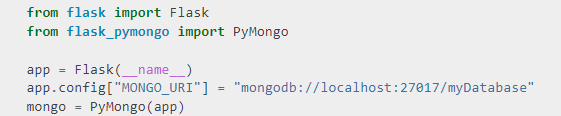
\includegraphics[width=12cm]{gambar/mongoDB3.png}
		\caption{Menambahkan Ekstensi PyMongo pada Flask. \\ Sumber: Dokumentasi PyMongo, https://flask-pymongo.readthedocs.io/en/latest/}
		\label{Gambar:registrasi blueprint}
	\end{figure}

	Inisialisasi MongoDB pada projek \emph{flask} dilakukan dengan menggunakan konstruktor PyMongo yang menerima objek app \emph{Flask} dan URI \emph{string} dari \emph{database} MongoDB. Setelah \emph{flask} dan MongoDB terintegrasi, fungsi-fungsi yang dapat kita lakukan adalah sebagai berikut:
	
	\begin{enumerate}
		\item Membuat Dokumen
		
		Metode PyMongo yang digunakan untuk menambahkan data ke dalam \emph{database} adalah db.\emph{collection}.\emph{insert\_one}() jika terdapat hanya satu data dan db.\emph{collection}.\emph{insert\_many}() jika terdapat lebih dari satu data. Untuk menambahkan dokumen ke dalam koleksi MongoDB, diperlukan untuk mendefinisikan \emph{dictionary} yang terdiri atas \emph{fields} dan \emph{values}.
		
			\begin{figure}[H]
				\centering
				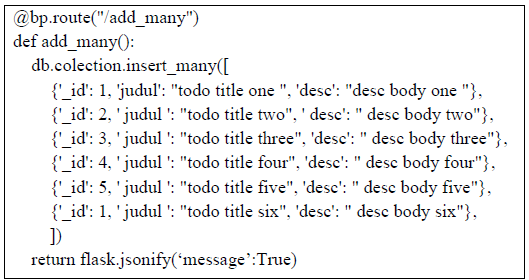
\includegraphics[width=12cm]{gambar/mongoDB4.png}
			\end{figure}
		
		Ketika mendefinisikan lebih dari satu data yang sama \emph{BulkWriteError} akan muncul, yang berarti hanya ada satu data yang terekam dan data lainnya yang sama akan hilang. Untuk mencegah hal tersebut, parameter \emph{ordered} pada fungsi \emph{insert\_many()} harus didefinisikan sebagai \emph{false} kemudian menangkap eksepsi \emph{BulkWriteError}.
		
		\item Membaca Dokumen
		
		\emph{Flask}-PyMongo memiliki beberapa metode dalam menerima data dari \emph{database}. Penerimaan semua dokumen dari koleksi menggunakan metode \emph{find()} untuk menerima semua data di \emph{database} dan \emph{find\_one()} untuk menerima satu data sesuai dengan ID yang diberikan. Metode \emph{find()} dapat menerima parameter yang digunakan sebagai \emph{filter}. Parameter \emph{filter} yang digunakan menjelaskan diksi yang mendefinisikan properti yang akan dicari.
		
		\item Memperbaharui dan Mengganti Dokumen
		
		Metode yang digunakan dalam memperbaharui data pada \emph{database} adalah \emph{update\_one()} atau \emph{replace\_one()}. Metode \emph{replace\_one()} mempunyai beberapa argumen sebagai berikut:
		
		\begin{enumerate}
			\item \emph{Filter}: berupa \emph{query} yang mendefinisikan data pada ID yang akan diganti,
			
			\item \emph{Replacement}: berupa data yang akan menggantikan data yang dihapus.
			
			\item \emph{Upsert}: adalah opsi \emph{boolean} yang jika dijadikan sebagai \emph{true} dapat membuat dokumen baru jika tidak terdapat target dokumen yang dimaksud.
			
		\end{enumerate}
	
	\item Menghapus Dokumen
	
	PyMongo menyediakan dua metode untuk menghapus satu atau lebih koleksi \emph{database} yaitu, \emph{delete\_one()} untuk menghapus satu koleksi dan \emph{delete\_many()} untuk menghapus beberapa koleksi.
	
	\begin{figure}[H]
		\centering
		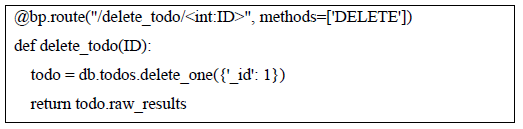
\includegraphics[width=12cm]{gambar/mongoDB5.png}
	\end{figure}

	Contoh kode di atas ketika menjalankan \emph{request} seperti http://\emph{localhost}:5000/\emph{delete}\_todo/5 PyMongo akan mencari entri berdasarkan ID yang diberikan dan menghapusnya.
	
	\item Menyimpan dan Menerima \emph{Files}
	
	MongoDB mengizinkan pengembang untuk menyimpan data biner ke dalam \emph{database} menggunakan spesifikasi GridFS. Ekstensi Flask-PyMongo menyediakan metode \emph{save\_file()} untuk menyimpan \emph{file} ke GridFS dan metode \emph{send\_file()} untuk menerima \emph{file} dari GridFS
	
	\begin{figure}[H]
		\centering
		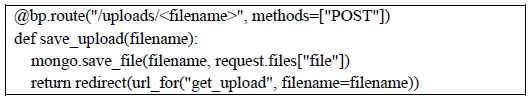
\includegraphics[width=12cm]{gambar/mongoDB6.png}
	\end{figure}
	
	Kode di atas, dibuat \emph{form} untuk menangani unggahan file dan mengembalikan nama \emph{file} yang telah terunggah.
		
	\end{enumerate}
	
\end{enumerate}

\section{Scrum}

\emph{Scrum} merupakan salah satu struktur kerja yang digunakan untuk mengembangkan produk. \emph{Scrum} diumumkan pertama kali oleh Ken Schwaber pada tahun 1995 pada konferensi Austin, namun fondasi metode \emph{scrum} sudah ada sejak tahun 1980 \citep{Oziera2016The}. \emph{Scrum} dibuat berdasarkan empirisme yang dicapai dengan beberapa kualitas. Hasil survei dari literatur, kualitas yang membangun empirisme \emph{scrum} adalah kejelasan dari setiap proses, inspeksi untuk mendeteksi masalah dan adaptasi terhadap perubahan

Setiap produk dihantarkan dengan cara yang fleksibel dan iteratif dalam kerangka kerja \emph{scrum} dimana setiap akhir \emph{sprint} terdapat produk nyata yang dapat dihantarkan. \emph{Requirement} yang dibutuhkan dalam suatu proyek berupa \emph{product backlog} yang diperbaharui secara berkala.

\emph{Scrum} mempunyai tiga elemen, di antaranya:

\begin{enumerate}
	\item \emph{Roles}
	
	\emph{Role} dalam \emph{scrum} terbagi menjadi empat \emph{role} utama, yaitu:
	
	\begin{enumerate}
		\item Tim \emph{Scrum}
		
		Tim \emph{scrum} merupakan kelompok kecil yang terdiri dari satu \emph{scrum master}, satu \emph{product owner}, dan pengembang. Pada tim \emph{scrum} tidak terdapat tim kecil ataupun hierarki. Seluruh anggota tim memiliki kemampuan penting untuk memberikan nilai ke dalam setiap \emph{sprint} dan fokus dengan satu tujuan pada satu waktu, \emph{product goal}.
		
		Tim \emph{scrum} bertanggung jawab dalam setiap aktivitas produk seperti kolaborasi dengan \emph{stakeholder}, \emph{maintenance}, verifikasi, \emph{research}, \emph{operation}, \emph{experimentation} dan pengembangan. Tim \emph{scrum} menghantarkan produk secara \emph{iterative} menggunakan \emph{sprint}, oleh karena itu tim \emph{scrum} juga bertanggung jawab untuk menciptakan nilai pada setiap \emph{sprint}-nya.
		
		\break
		
		\item \emph{Scrum Master}
		
		\emph{Scrum master} memiliki tanggung jawab dalam merealisasikan \emph{scrum} yang terdefinisi pada panduan \emph{scrum}. Setiap anggota tim dibantu \emph{scrum master} untuk mengerti bagaimana teori dan praktik kerangka kerja pada metode \emph{scrum}. Selain itu, menjaga efektivitas dari tim \emph{scrum} juga menjadi tanggung jawab \emph{scrum master}.
		
		\item \emph{Product Owner}
		
		\emph{Product owner} memiliki tanggung jawab untuk meningkatkan nilai komersial produk yang dihasilkan oleh \emph{development team} dan mengelola \emph{product backlog} agar lebih maksimal. Hanya \emph{product owner} yang memiliki tanggung jawab untuk mengelola \emph{product backlog}. Adapun pengelolaan \emph{product backlog}:
		
		\begin{enumerate}
			\item Penyampaian isi \emph{product backlog}.
			\item Memastikan \emph{development team} memahami \emph{product backlog}.
			\item Memastikan isi daripada \emph{product backlog} transparan dan jelas bagi seluruh anggota tim.
			\item Mengurutkan item pada \emph{product backlog} untuk mencapai tujuan secara optimal.
			
		\end{enumerate}
	
		\item \emph{Development Team}
		
		\emph{Development team} atau tim pengembang adalah profesional yang mengeksekusi isi yang tercantum di dalam \emph{product backlog}. Tim Pengembang berkomitmen untuk membuat semua aspek \emph{increment} yang dapat berfungsi pada setiap \emph{sprint}. Namun, tim Pengembang juga selalu bertanggung jawab untuk:
		
		\begin{enumerate}
			\item Membuat rancangan \emph{sprint} atau dikenal dengan \emph{sprint backlog}.
			\item Membuat definisi penyelesaian sebuah \emph{task}.
			\item Mengadaptasikan semua \emph{plan} setiap hari sampai \emph{sprint goal}.
			\item Mengurutkan \emph{item} pada \emph{product backlog} untuk mencapai tujuan secara optimal.
			
		\end{enumerate}
		
	\end{enumerate}
	
	\item \emph{Artifacts}
	
	Artefak \emph{scrum} dirancang untuk memaksimalkan transparansi informasi utama dan kesempatan untuk menginspeksi dan mengadaptasi.
	
	\begin{enumerate}
		\item \emph{Product Backlog}
		
		\emph{Product backlog} atau umumnya disebut dengan \emph{user stories} merupakan kumpulan fitur-fitur yang terdapat pada suatu produk . \emph{User stories} dapat ditambahkan, dimodifikasi, atau dihilangkan dari \emph{product backlog} selama proyek berjalan.
		
		\item \emph{Sprint Backlog}
		
		\emph{Sprint backlog} adalah beberapa \emph{user stories} yang diambil dari \emph{product backlog} untuk dijalankan pada satu \emph{sprint}. \emph{Sprint backlog} mencakup seluruh kegiatan kerja yang diperlukan untuk mencapai \emph{sprint goal}.
		
		Pada satu \emph{sprint} terdapat \emph{increment} yang merupakan manifestasi dari \emph{user stories} yang diselesaikan dan total \emph{increment} dari seluruh \emph{sprint} sebelumnya.
		
	\end{enumerate}
	
	\item Events
	
	\emph{Event} merupakah wadah dari semua \emph{event} yang terdapat pada \emph{scrum}. \emph{Event} dibuat sebagai perwujudan salah satu dari tiga pilar \emph{scrum}. Seluruh \emph{event} berjalan secara bersamaan untuk mengurangi kompleksitas.
	
		\begin{enumerate}
		\item \emph{Sprint}
		
		\emph{Sprint} adalah komponen utama kerangka kerja \emph{scrum}, dimana sebuah ide menjadi sebuah nilai. Lama durasi \emph{sprint} bersifat tetap yaitu satu hingga empat minggu untuk menjaga konsistensi.
		
		\emph{Sprint} berfokus untuk menghantarkan beberapa \emph{user stories} pada \emph{product backlog}. Setiap satu \emph{sprint} memiliki beberapa kegiatan diantaranya \emph{sprint planning}, \emph{sprint review} dan \emph{sprint retrospective}.
		
		\item \emph{Sprint Planning}
		
		\emph{Sprint backlog} adalah beberapa \emph{user stories} yang diambil dari \emph{product backlog} untuk dijalankan pada satu \emph{sprint}. \emph{sprint backlog} mencakup semua kegiatan kerja yang dibutuhkan untuk mencapai \emph{sprint goal}.
		
		Sebelum memulai \emph{sprint}, perencanaan apa yang akan dilaksanakan pada saat \emph{sprint} dilakukan pada saat \emph{sprint planning} oleh seluruh anggota tim \emph{scrum}. Waktu untuk melaksanakan \emph{sprint planning} terbatas dengan lama durasi hingga delapan jam. Fungsi dari \emph{sprint planning} adalah memutuskan apa yang dapat dimasukkan ke dalam \emph{increment} dari \emph{sprint} dan bagaimana penyelesaian yang dibutuhkan untuk menghantarkan \emph{increment}.
		
		\item \emph{Daily Scrum}
		
		\emph{Daily scrum} adalah kegiatan 15 menit bagi para pengembang untuk memeriksa perkembangan menuju \emph{sprint goal} dan menyesuaikan pekerjaan yang akan dikerjakan selama 24 jam ke depan. Pada kegiatan \emph{daily scrum}, hal apa saja yang akan dikerjakan hari ini, apa yang telah dikerjakan kemarin dan hambatan yang telah dialami dalam mencapai \emph{sprint goal} akan didiskusikan oleh tim pengembang.
		
		\break
		\item \emph{Sprint Review}
		
		Tahap ini dilaksanakan pada akhir \emph{sprint}, tujuannya untuk mengawasi apa yang telah diselesaikan di \emph{sprint}. Menurut hasil tinjauan serta perubahan \emph{product backlog}, tim \emph{scrum} menentukan kembali pekerjaan selanjutnya yang dapat mengoptimalkan produk.
		
		\emph{Sprint review} bersifat informal dan diselenggarakan dengan lama durasi empat jam untuk sprint dalam waktu satu bulan. Semakin singkat durasi \emph{sprint}, maka semakin singkat juga durasi \emph{sprint review}.
		
	\end{enumerate}
	
\end{enumerate}

\begin{comment}
\section{Studi Banding Sistem Informasi Rumah Sakit}

Dalam melakukan studi banding, peneliti menggunakan 3 jurnal yang didapat dari internet. Jurnal pertama peneliti ambil dari penelitian yang dilakukan oleh Ardiansyah dengan judul "Analisis dan Perancangan Sistem Informasi Manajemen Rumah Sakit Berbasis \emph{Website} Pada Rumah Sakit Umum Kambang Kota Jambi". \citep{Ardiansyah2021analisis:10}. Jurnal kedua peneliti ambil dari jurnal yang berjudul "Sistem Informasi Rekam Medis Pada Rumah Sakit Umum Daerah (RSUD) Pacitan Berbasis \emph{Web Base}" oleh Gunawan Susanto. \citep{Gunawan2011sistem:11}. Dan Jurnal Ketiga peneliti ambil dari penelitian yang dilakukan oleh Inah Carminah dengan judul "Aplikasi Monitoring Perawatan Luka Diabetes Melitus Berbasis \emph{Website}". \cite{Carminah2021aplikasi:12}.

\subsection{Studi Banding Berdasarkan Fitur}
Berikut diagram \emph{use case} dari ketiga jurnal yang telah peneliti sebutkan di atas.

\begin{enumerate}
	\item Diagram \emph{use case} pada jurnal pertama
	
	Diagram \emph{use case} ada pada halaman berikutnya pada \textbf{Gambar 2.1}
	\begin{figure}[H]
		\centering
		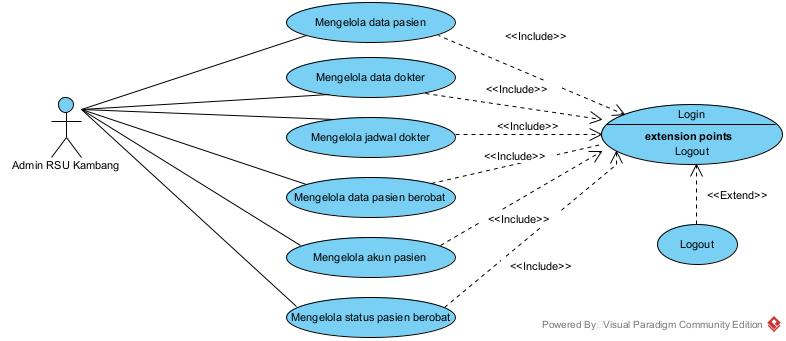
\includegraphics[width=12cm]{gambar/jurnal1_use_case_admin.jpg}
		\caption{Diagram \emph{use case} admin jurnal pertama \\ Sumber: \citep{Ardiansyah2021analisis:10}} 
		\label{Gambar:usecaseadminjurnalpertama}
	\end{figure}
	
	\begin{figure}[H]
		\centering
		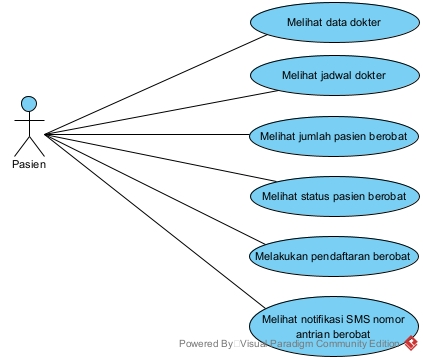
\includegraphics[width=12cm]{gambar/jurnal1_use_case_pasien.jpg}
		\caption{Diagram \emph{use case} pasien jurnal pertama \\ Sumber: \citep{Ardiansyah2021analisis:10}}
		\label{Gambar:usecasepasienjurnalpertama}
	\end{figure}
	
	\item \emph{Data flow diagram}(DFD) pada jurnal kedua.
	
	Pada jurnal kedua tidak ditemukan \emph{use case} diagram dan hanya tersedia \emph{data flow diagram}. Berikut \emph{data flow diagram} pada jurnal kedua.
	
	\begin{figure}[H]
		\centering
		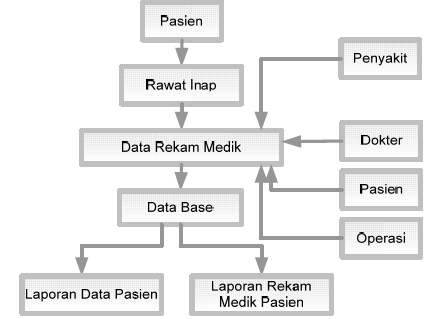
\includegraphics[width=8cm]{gambar/data_flow_diagram_jurnal2.png}
		\caption{Diagram \emph{data flow diagram} jurnal kedua \\ Sumber: \citep{Gunawan2011sistem:11}}
		\label{Gambar:dataflowdiagramjurnalkedua}
	\end{figure}
	
	\item Diagram \emph{use case} pada jurnal ketiga
	
	\begin{figure}[H]
		\centering
		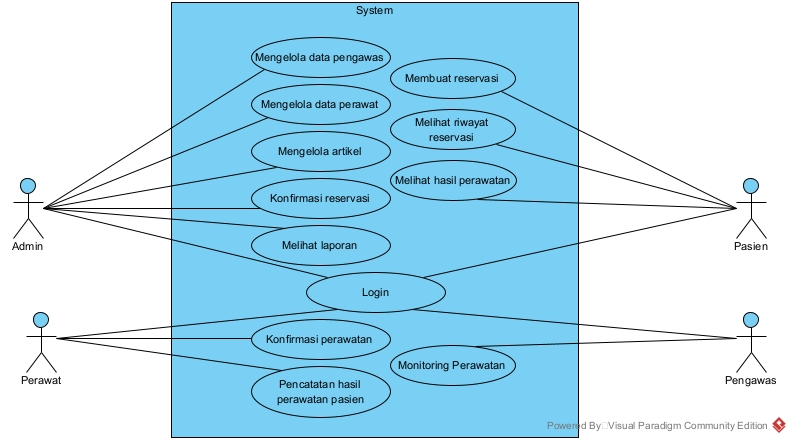
\includegraphics[width=12cm]{gambar/diagram_use_case_jurnal3.jpg}
		\caption{Diagram \emph{use case} jurnal ketiga \\ Sumber: \citep{Carminah2021aplikasi:12}}
		\label{Gambar:usecasejurnalketiga}
	\end{figure}
	
\end{enumerate}

\subsection{Studi Banding Berdasarkan UI/UX}

\begin{enumerate}
	\item UI/UX pada jurnal pertama
	
	Berikut di bawah ini merupakan UI/UX yang ditampilkan didalam jurnal pertama: 
	
	\textbf{Gambar 2.5} menampilkan rancangan halaman utama registrasi \emph{online} RSU Kambang yang berisi sosial media, dan alamat beserta tombol menu.
	
	\begin{figure}[H]
		\centering
		
\includegraphics[width=12cm]{gambar/halaman_utama_registrasi_online.png}
		\caption{Rancangan halaman registrasi \emph{online} \\ Sumber: \citep{Ardiansyah2021analisis:10}}
		\label{Gambar:halamanutamaregistrasionline}
	\end{figure}
	
	\begin{figure}[H]
		\centering
		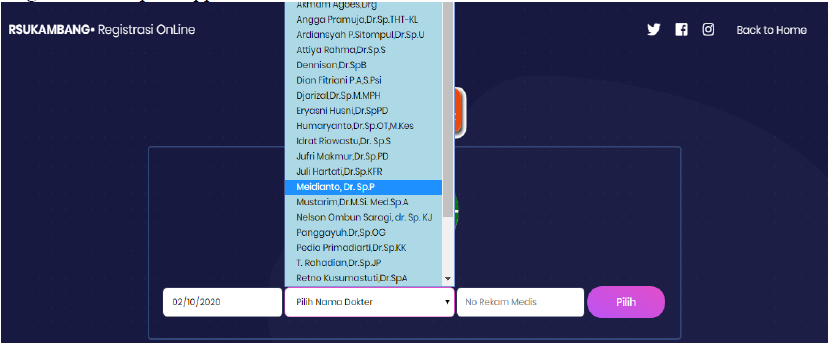
\includegraphics[width=12cm]{gambar/halaman_pilih_appointment.png}
		\caption{Rancangan Halaman pilih \emph{appointment} \\ Sumber: \citep{Ardiansyah2021analisis:10}}
		\label{Gambar:halamanpilihappointment}
	\end{figure}
	
	\textbf{Gambar 2.6} menampilkan rancangan halaman \emph{appointment} RSU Kambang yang berisi \emph{field} tanggal \emph{appointment}, \emph{field} nama dokter yang dituju, \emph{field} nomor rekam medis, sosial media, tombol pilih dan tombol \emph{back to home}.
	
	\textbf{Gambar 2.7} pada halaman selanjutnya menampilkan rancangan daftar pasien yang sudah mendaftar berobat RSU Kambang yang berisi tanggal, nama dokter, sosial media, tombol \emph{back to home}. Lalu ada tabel berupa nomor, nomor rekam medis, nama pasien, nomor antrian, dan status beserta tombol daftar shift pagi dan shift siang.
	
	\begin{figure}[H]
		\centering
		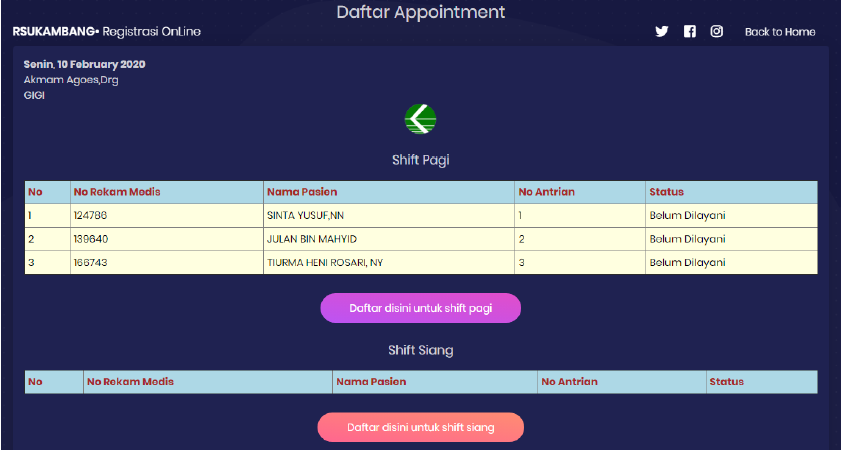
\includegraphics[width=12cm]{gambar/halaman_tampil_daftar_pasien_mendaftar.png}
		\caption{Rancangan halaman daftar pasien yang sudah mendaftar berobat \\ Sumber: \citep{Ardiansyah2021analisis:10}}
		\label{Gambar:halamandaftarpasienyangsudahmendaftar}
	\end{figure}
	
	\begin{figure}[H]
		\centering
		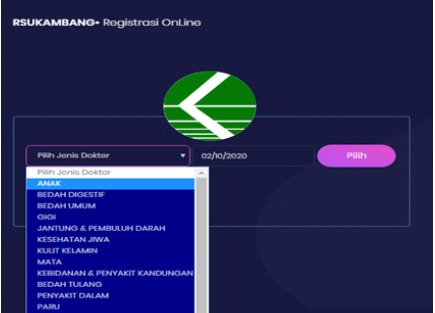
\includegraphics[width=10cm]{gambar/halaman_jadwal_dokter.png}
		\caption{Rancangan halaman jadwal dokter \\ Sumber: \citep{Ardiansyah2021analisis:10}}
		\label{Gambar:halamanjadwaldokter}
	\end{figure}
	
	\textbf{Gambar 2.8} pada halaman sebelumnya menampilkan rancangan halaman jadwal dokter yang berisi \emph{field} pilih jenis dokter dan \emph{field} tanggal beserta tombol pilih.
	
	\textbf{Gambar 2.9} menampilkan rancangan halaman \emph{input} registrasi berobat yang berisi \emph{field} nama dokter, \emph{field} nomor rekam medis, \emph{field} nama pasien, \emph{field} pilihan pendaftaran, \emph{field} nomor \emph{handphone}, \emph{field} tanggal lahir, \emph{field} jam registrasi berobat beserta \emph{field} tanggal registrasi berobat.
	
	\begin{figure}[H]
		\centering
		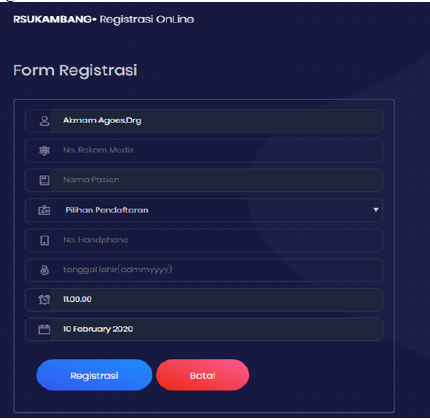
\includegraphics[width=10cm]{gambar/halaman_input_registrasi.png}
		\caption{Rancangan halaman \emph{input} registrasi berobat \\ Sumber: \citep{Ardiansyah2021analisis:10}}
		\label{Gambar:halamaninputregistrasiobat}
	\end{figure}
	
	\textbf{Gambar 2.10} pada halaman selanjutnya menampilkan rancangan halaman utama admin yang berisi ucapan selamat datang, foto RSU Kambang Jambi, beserta tombol pengaturan.
	
	\begin{figure}[H]
		\centering
		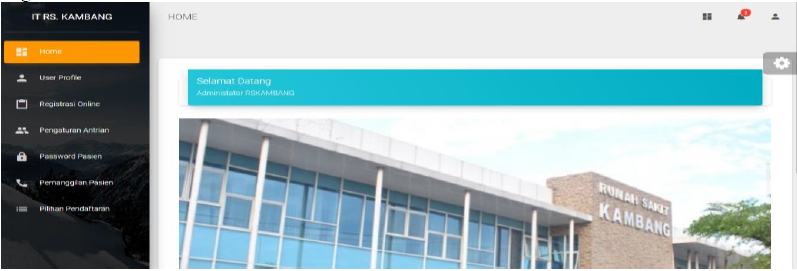
\includegraphics[width=12cm]{gambar/halaman_utama_admin.png}
		\caption{Rancangan halaman utama admin \\ Sumber: \citep{Ardiansyah2021analisis:10}}
		\label{Gambar:halamanutamaadmin}
	\end{figure}
	
	\textbf{Gambar 2.11} menampilkan rancangan halaman \emph{user profile} yang berisi tombol pengaturan, dan tabel Data Login Admin yang berisi \emph{username}, nama, Jabatan, No. HP, Email, Status, dan Opsi.
	
	\begin{figure}[H]
		\centering
		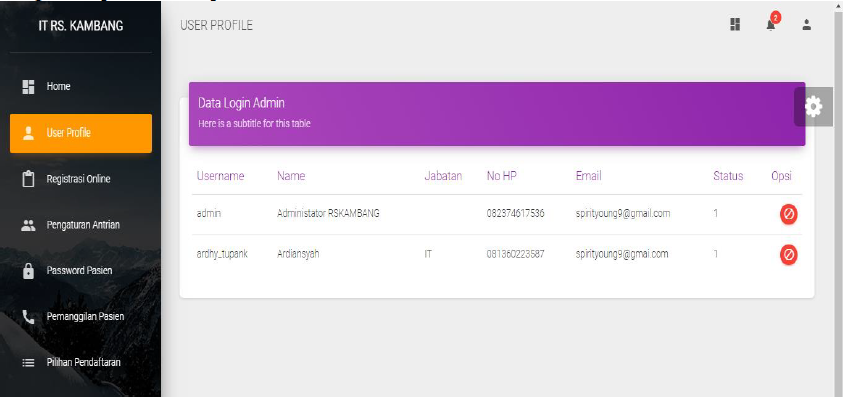
\includegraphics[width=12cm]{gambar/halaman_tampil_data_user_profile.png}
		\caption{Rancangan halaman \emph{user profile} \\ Sumber: \citep{Ardiansyah2021analisis:10}}
		\label{Gambar:halamanuserprofile}
	\end{figure}
	
	\textbf{Gambar 2.12} pada halaman selanjutnya menampilkan rancangan halaman \emph{user} yang melakukan registrasi \emph{online} yang berisi \emph{field} tanggal, tombol pilih, tombol pengaturan, tabel data registrasi pasien yang berisi Nama Daftar, No. RM, No. HP, Tanggal Registrasi, Tanggal Berobat, Status, Nama Dokter, dan Aksi.
	
	\begin{figure}[H]
		\centering
		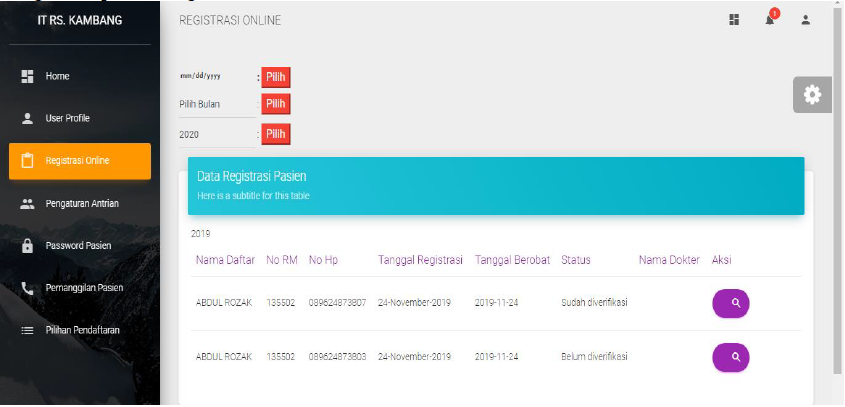
\includegraphics[width=12cm]{gambar/halaman_tampil_data_registrasi_online.png}
		\caption{Rancangan halaman \emph{list user} melakukan registrasi \emph{online} \\ Sumber: \citep{Ardiansyah2021analisis:10}}
		\label{Gambar:halamanusermelakukanregistrasi}
	\end{figure}
	
	\textbf{Gambar 2.13} menampilkan rancangan halaman detail data \emph{user} yang melakukan registrasi \emph{online} yang berisi tabel data registrasi antrian berupa No. RM, Nama, Tanggal Lahir, No. Telephone, Tanggal Registrasi, No. HP, Status, dan No. Antrian. Terdapat tabel informasi dokter yang dituju berupa Nama Dokter, Status Dokter, Jam Dokter, Tanggal Berobat, dan Poliklinik. Tabel \emph{cancel} berupa status antrian dan keterangan. Dan ada tombol pengaturan.
	
	\begin{figure}[H]
		\centering
		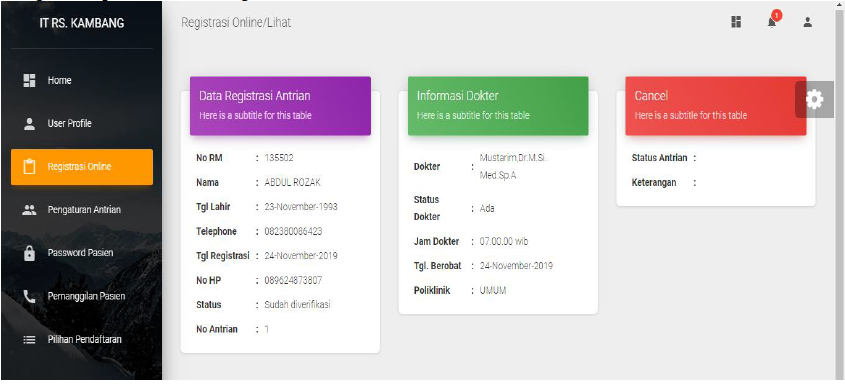
\includegraphics[width=12cm]{gambar/halaman_tampil_detail_data_registrasi_online.png}
		\caption{Rancangan halaman detail data \emph{user} melakukan registrasi \emph{online} \\ Sumber: \citep{Ardiansyah2021analisis:10}}
		\label{Gambar:halamandetaildatausermelakukanregistrasionline}
	\end{figure}
	
	\textbf{Gambar 2.14} pada halaman selanjutnya menampilkan rancangan halaman tampil daftar alasan \emph{cancel} registrasi yang berisi tabel alasan \emph{cancel} registrasi berupa Nomor, alasan, tombol tambah data, edit dan hapus.
	
	\begin{figure}[H]
		\centering
		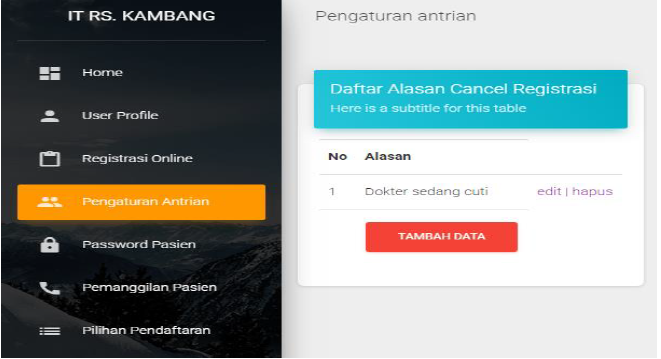
\includegraphics[width=10cm]{gambar/halaman_tampil_daftar_alasan_cancel_registrasi.png}
		\caption{Rancangan halaman daftar alasan \emph{cancel} registrasi \\ Sumber: \citep{Ardiansyah2021analisis:10}}
		\label{Gambar:halamandaftaralasancancelregistrasi}
	\end{figure}
	
	Berikut merupakan tampilan UI/UX live pada website  \emph{live} RSU Kambang Jambi pada \url{https://rsukambang.com/}
	
	\begin{figure}[H]
		\centering
		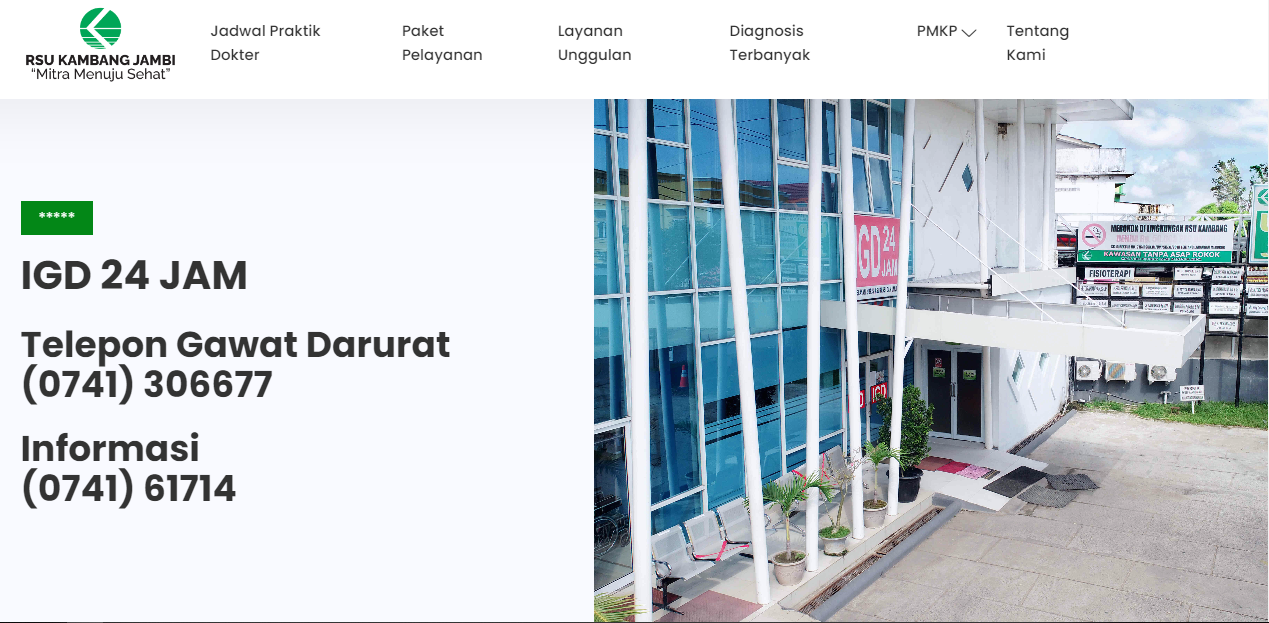
\includegraphics[width=12cm]{gambar/halaman_utama_rsu_kambang_jambi_live.png}
		\caption{halaman utama RSU Kambang \emph{live} \\ Sumber: \url{https://rsukambang.com/}}
		\label{Gambar:halamanutamarsukambanglive}
	\end{figure}
	
	\textbf{Gambar 2.15} menampilkan halaman utama RSU Kambang \emph{live} yang berisi informasi nomor \emph{telephone}, visi, misi, info pelayanan, daftar berobat via whatsapp. (\textbf{Gambar 2.16}) pada halaman berikutnya berisi info asuransi yang diterima, dan lokasi RS.
	
	\begin{figure}[H]
		\centering
		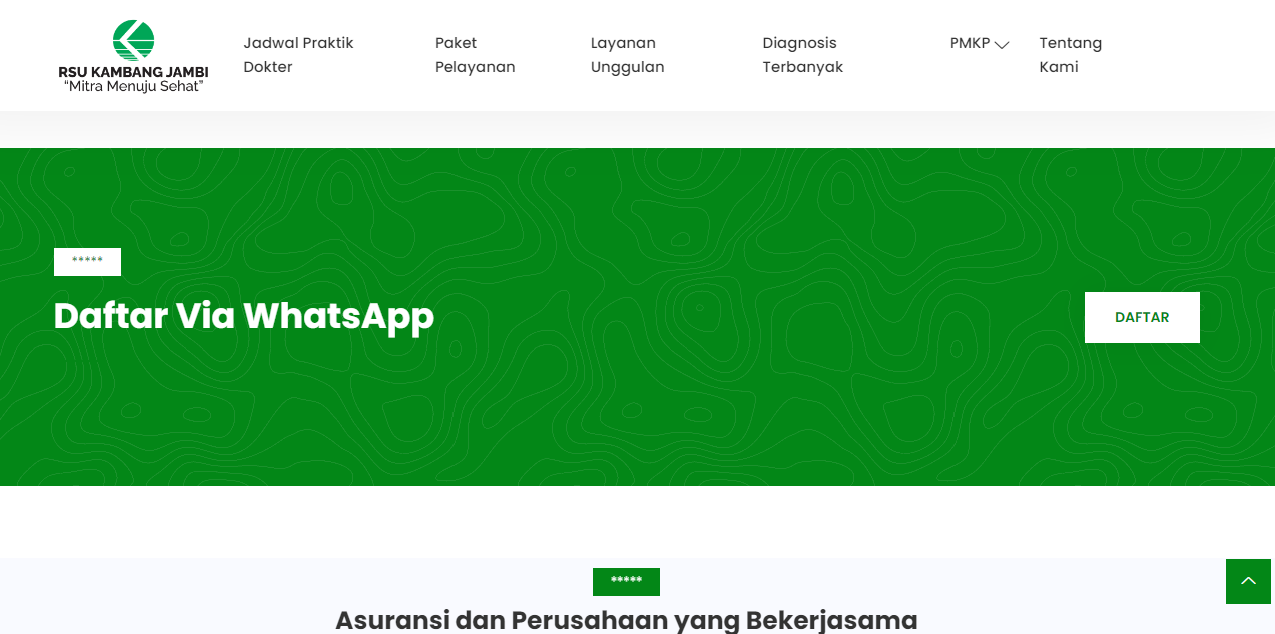
\includegraphics[width=12cm]{gambar/halaman_utama_lanjutan_daftar_berobat_live.png}
		\caption{halaman utama RSU Kambang \emph{live} lanjutan \\ Sumber: \url{https://rsukambang.com/}}
		\label{Gambar:halamanutamarsukambanglivelanjutan}
	\end{figure}
	
	\textbf{Gambar 2.17} menampilkan halaman jadwal praktik dokter \emph{live} yang berisi \emph{flyer} jadwal praktik dokter.
	
	\begin{figure}[H]
		\centering
		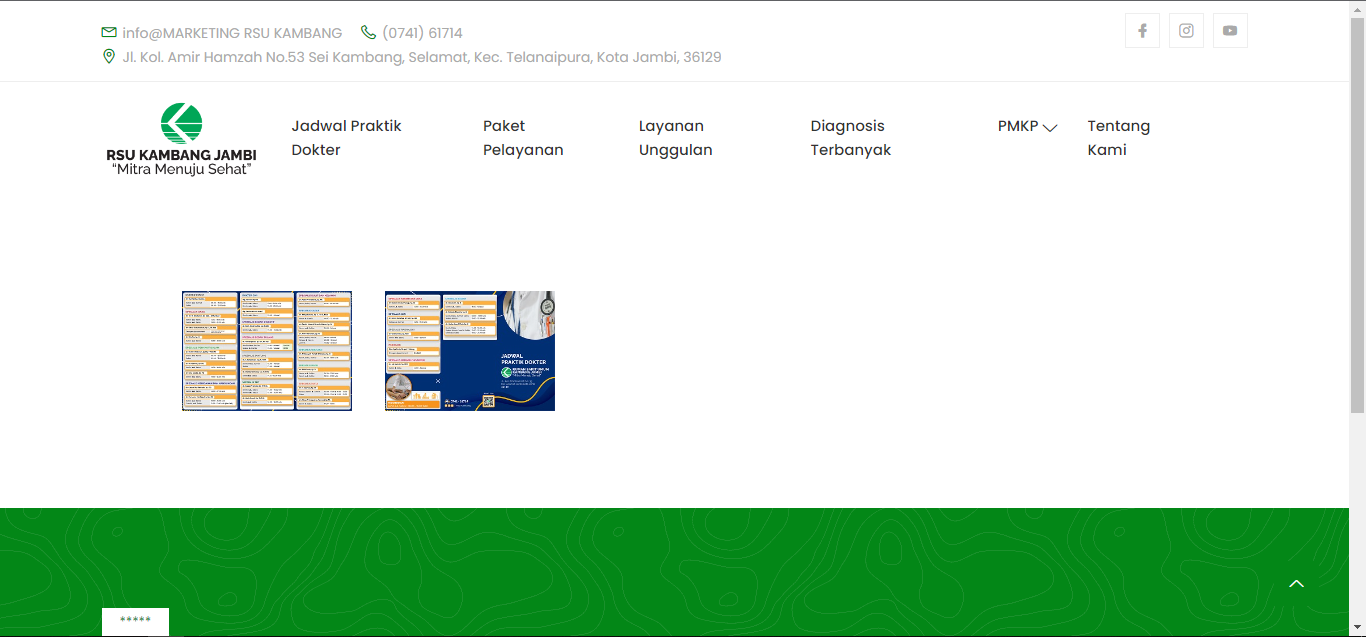
\includegraphics[width=12cm]{gambar/halaman_jadwal_praktik_dokter_rsu_kambang_live.png}
		\caption{halaman jadwal praktik dokter \emph{live} \\ Sumber: \url{https://rsukambang.com/}}
		\label{Gambar:halamanjadwalpraktikdokterlive}
	\end{figure}
	
	\textbf{Gambar 2.18} pada halaman selanjutnya menampilkan halaman paket pelayanan \emph{live} yang berisi flyer paket pelayanan beserta harganya.
	
	\begin{figure}[H]
		\centering
		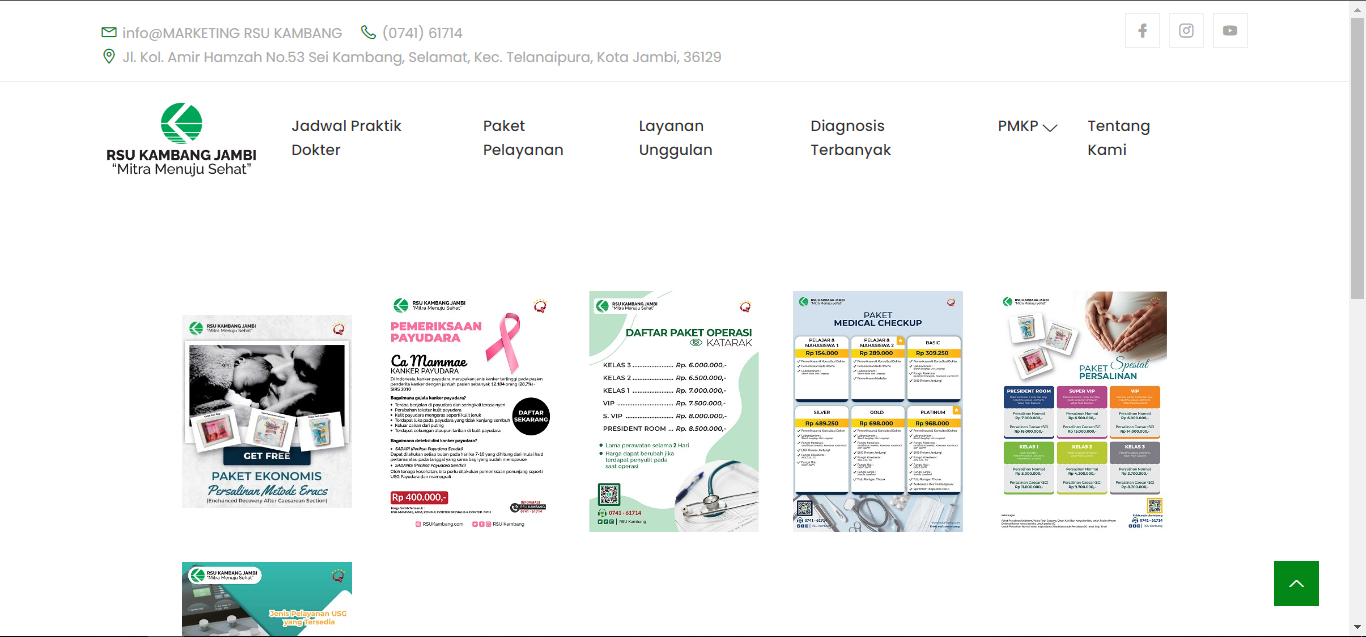
\includegraphics[width=12cm]{gambar/halaman_paket_pelayanan_live.png}
		\caption{halaman paket pelayanan \emph{live} \\ Sumber: \url{https://rsukambang.com/}}
		\label{Gambar:halamanpaketpelayananlive}
	\end{figure}
	
	
	\textbf{Gambar 2.19} menampilkan halaman layanan unggulan \emph{live} yang berisi daftar pelayanan dan penunjang medis beserta daftar sarana dan prasarana yang ada di RSU Kambang.
	
	\begin{figure}[H]
		\centering
		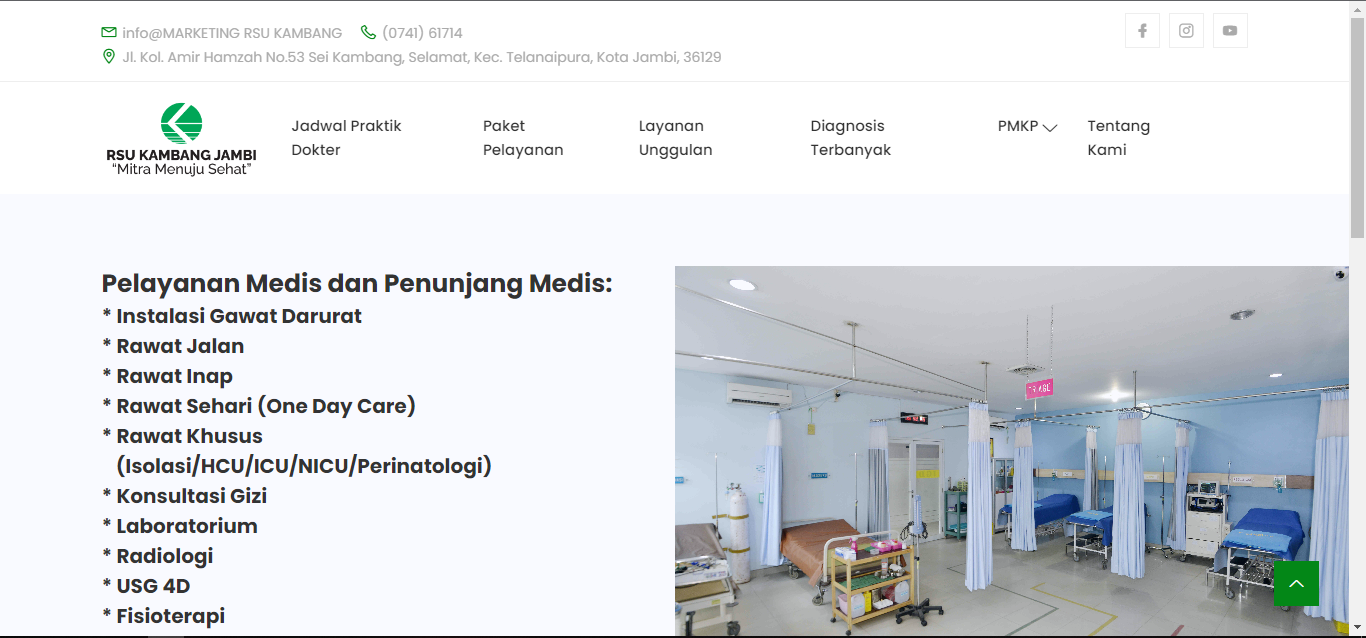
\includegraphics[width=12cm]{gambar/halaman_layanan_unggulan_live.png}
		\caption{halaman layanan unggulan \emph{live} \\ Sumber: \url{https://rsukambang.com/}}
		\label{Gambar:halamanlayananunggulanlive}
	\end{figure}
	
	\textbf{Gambar 2.20} pada halaman berikutnya menampilkan halaman diagnosis terbanyak \emph{live} yang berisis tabel daftar 10 Besar Penyakit Rawat Jalan Tahun 2022 dan tabel daftar 10 Besar Penyakit Rawat Inap Tahun 2022.
	
	\begin{figure}[H]
		\centering
		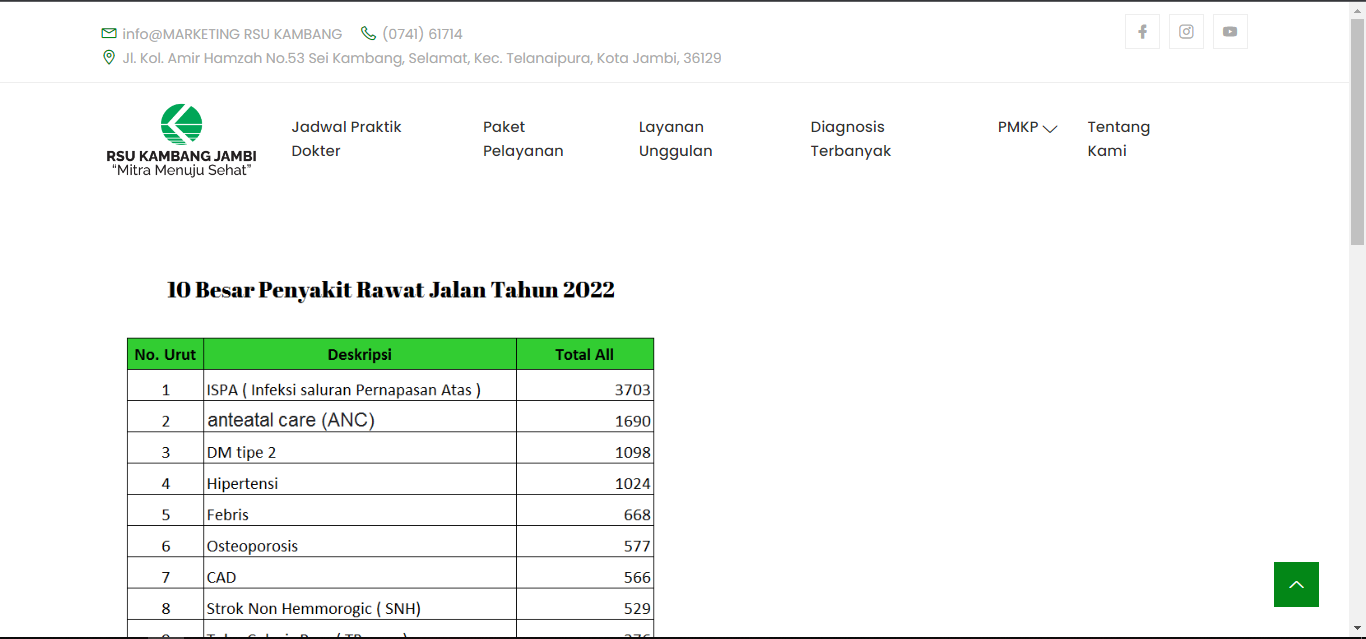
\includegraphics[width=12cm]{gambar/halaman_diagnosis_terbanyak_live.png}
		\caption{halaman diagnosis terbanyak \emph{live} \\ Sumber: \url{https://rsukambang.com/}}
		\label{Gambar:halamandiagnosisterbanyaklive}
	\end{figure}
	
	\textbf{Gambar 2.21} menampilkan halaman PKMP \emph{live} yang berisi 13 indikator nasional mutu dalam bentuk grafik.
	
	\begin{figure}[H]
		\centering
		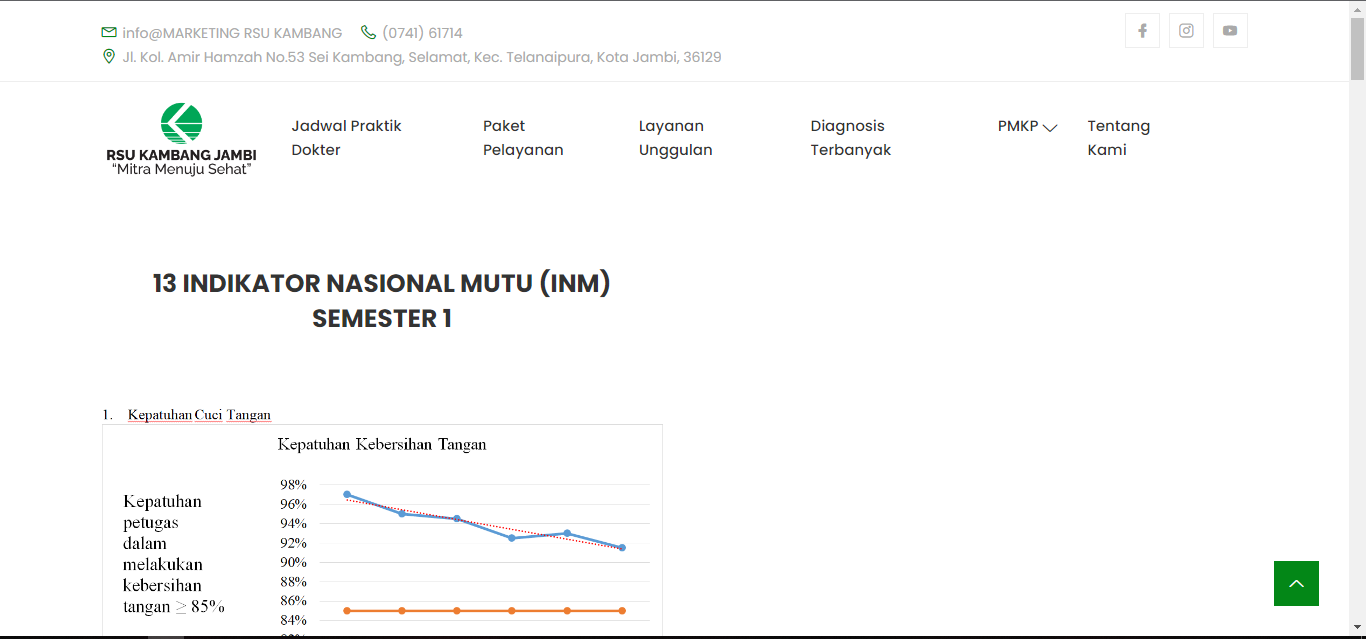
\includegraphics[width=12cm]{gambar/halaman_pkmp_live.png}
		\caption{halaman pkmp \emph{live} \\ Sumber: \url{https://rsukambang.com/}}
		\label{Gambar:halamanpkmplive}
	\end{figure}
	
	\textbf{Gambar 2.22} pada halaman selanjutnya menampilkan halaman tentang kami \emph{live} yang berisi profil, visi, dan misi RSU Kambang Jambi.
	
	\begin{figure}[H]
		\centering
		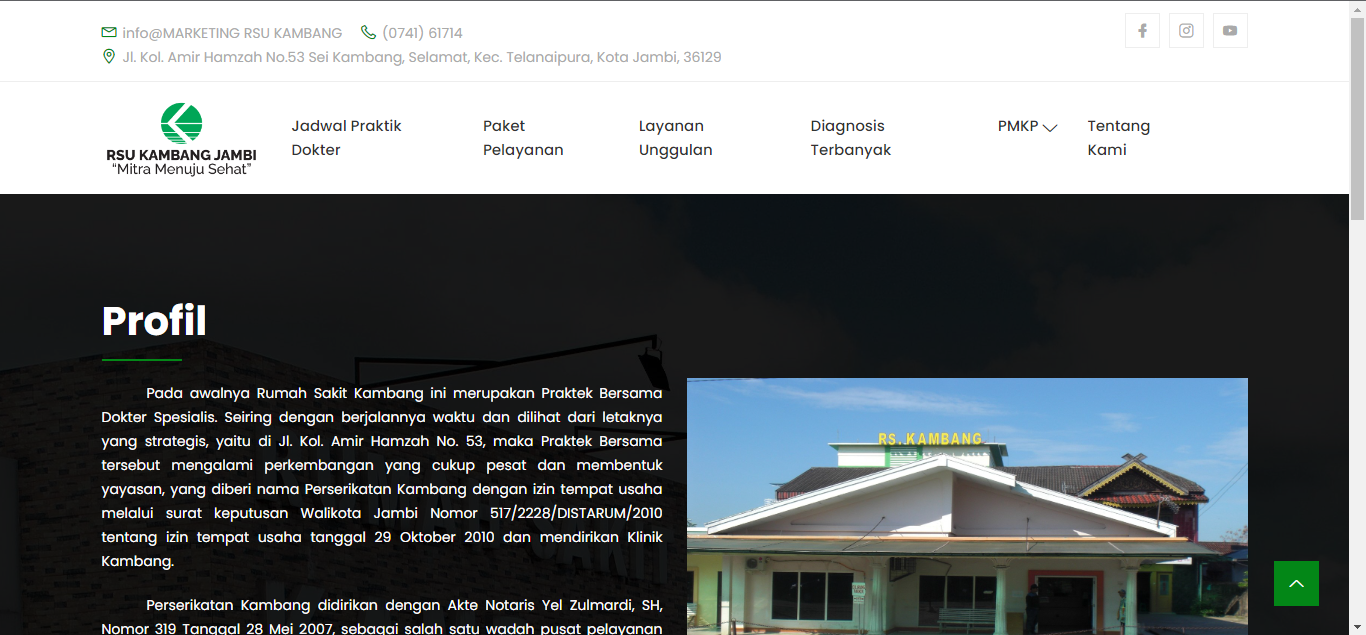
\includegraphics[width=12cm]{gambar/halaman_tentang_kami_live.png}
		\caption{halaman tentang kami \emph{live} \\ Sumber: \url{https://rsukambang.com/}}
		\label{Gambar:halamantentangkamilive}
	\end{figure}
	
	\item UI/UX pada jurnal kedua
	
	Berikut di bawah ini merupakan UI/UX yang ditampilkan didalam jurnal kedua:
	
	\begin{figure}[H]
		\centering
		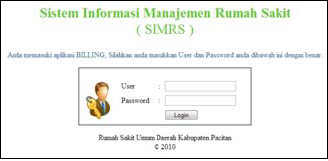
\includegraphics[width=12cm]{gambar/halaman_login.png}
		\caption{Rancangan halaman \emph{login} Sistem Informasi Manajemen Rumah Sakit \\ Sumber: \citep{Gunawan2011sistem:11}}
		\label{Gambar:halamanloginsisteminformasimanajemenrumahsakit}
	\end{figure}
	
	\textbf{Gambar 2.23} menampilkan rancangan halaman \emph{login} Sistem Informasi Manajemen Rumah Sakit yang berisi \emph{field} user dan \emph{field password} beserta tombol login.
	
	\begin{figure}[H]
		\centering
		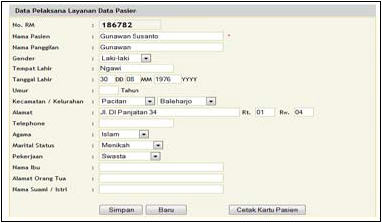
\includegraphics[width=12cm]{gambar/halaman_petugas_mendaftarkan_pasien.png}
		\caption{Rancangan halaman daftar pasien \\ Sumber: \citep{Gunawan2011sistem:11}}
		\label{Gambar:halamandaftarpasien}
	\end{figure}
	
	\textbf{Gambar 2.24} menampilkan rancangan halaman daftar pasien yang berisi \emph{field} No. RM, \emph{field} nama pasien, \emph{field} nama panggilan, \emph{field} gender, \emph{field} tempat lahir, \emph{field} tanggal lahir, \emph{field} umur, \emph{field} kecamatan/kelurahan, \emph{field} alamat/rt/rw, \emph{field telephone}, \emph{field} agama, \emph{field} marital status, \emph{field} pekerjaan, \emph{field} nama ibu, \emph{field} alamat orang tua, \emph{field} nama suami/istri,  beserta tombol simpan, baru, dan cetak kartu pasien.
	
	\begin{figure}[H]
		\centering
		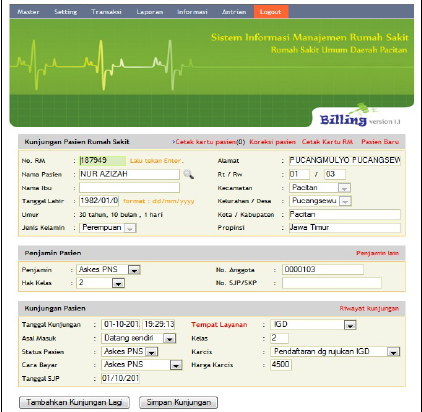
\includegraphics[width=8cm]{gambar/halaman_petugas_mengunjungkan_pasien_ke_poli.png}
		\caption{Rancangan halaman petugas mengunjungkan pasien ke poliklinik. \\ Sumber: \citep{Gunawan2011sistem:11}}
		\label{Gambar:halamanpetugasmengunjungkanpasienkepoliklinik}
	\end{figure}
	
	\textbf{Gambar 2.25} menampilkan rancangan halaman petugas mengunjungkan pasien ke poliklinik yang berisi tabel kunjungan pasien rumah sakit berisi \emph{field} No. RM, \emph{field} nama pasien, \emph{field} nama ibu, \emph{field} tanggal lahir, \emph{field} umur, \emph{field} jenis kelamin, \emph{field} alamat, \emph{field} rt/rw, \emph{field} kecamatan, \emph{field} kelurahan/desa, \emph{field} kota/kabupaten, dan \emph{field} provinsi. Lalu ada tabel penjamin pasien berisi \emph{field} penjamin, \emph{field} hak kelas, \emph{field} No. Anggota, \emph{field} No. SJP/SKP. Dan tabel kunjungan pasien berisi \emph{field} tanggal kunjungan, \emph{field} asal masuk, \emph{field} status pasien, \emph{field} cara bayar, \emph{field} tanggal SJP, \emph{field} tempat pelayanan, \emph{field} kelas, \emph{field} karcis, dan \emph{field} harga karcis. beserta tombol tambahkan kunjungan lagi dan simpan kunjungan.
	
	\begin{figure}[H]
		\centering
		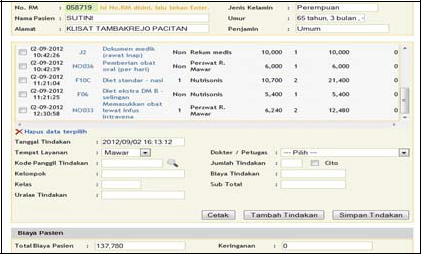
\includegraphics[width=12cm]{gambar/halaman_pembuatan_tagihan_billing.png}
		\caption{Rancangan halaman pembuatan tagihan billing. \\ Sumber: \citep{Gunawan2011sistem:11}}
		\label{Gambar:halamanpembuatantagihanbilling}
	\end{figure}
	
	\textbf{Gambar 2.26} menampilkan rancangan halaman pembuatan tagihan billing yang berisi \emph{field} No. RM, \emph{field} nama pasien, \emph{field} alamat, \emph{field} jenis kelamin, \emph{field} umur, \emph{field} penjamin, \emph{field} pilihan layanan atau barang yang digunakan, \emph{field} tanggal tindakan, \emph{field} tempat layanan, \emph{field} kode panggil tindakan, \emph{field} kelompok, \emph{field} kelas, \emph{field} uraian tindakan, \emph{field} dokter/petugas, \emph{field} jumlah tindakan, \emph{field} biaya tindakan, \emph{field} subtotal, \emph{field} total biaya pasien, \emph{field} keringanan beserta tombol cetak, tambah tindakan, dan simpan tindakan.
	
	\textbf{Gambar 2.27} pada halaman berikutnya menampilkan rancangan halaman pengelompokan penyakit berdasarkan icd yang berisi \emph{field} kode diagnosis ICD, \emph{field} diagnosis ICD, \emph{field} search, dan \emph{field} daftar penyakit beserta tombol tambah, koreksi, dan hapus.
	
	\begin{figure}[H]
		\centering
		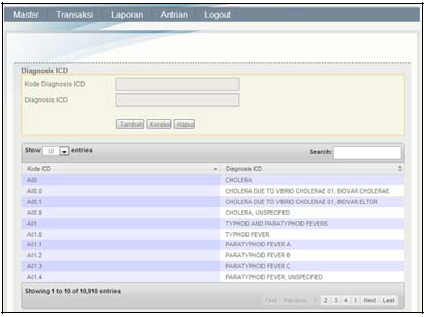
\includegraphics[width=12cm]{gambar/halaman_pengelompokan_penyakit_icd.png}
		\caption{Rancangan halaman pengelompokan penyakit berdasarkan ICD. \\ Sumber: \citep{Gunawan2011sistem:11}}
		\label{Gambar:halamanpengelompokanpenyakitberdasarkanicd}
	\end{figure}
	
	\begin{figure}[H]
		\centering
		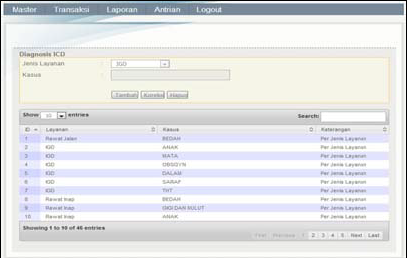
\includegraphics[width=12cm]{gambar/halaman_pengelompokan_kasus_penyakit_berdasarkan_poli.png}
		\caption{Rancangan halaman pengelompokan kasus penyakit berdasarkan poliklinik. \\ Sumber: \citep{Gunawan2011sistem:11}}
		\label{Gambar:halamanpengelompoankasuspenyakitberdasarkanpoliklinik}
	\end{figure}
	
	\textbf{Gambar 2.28} menampilkan rancangan halaman pengelompokan kasus penyakit berdasarkan poliklinik yang berisi \emph{field} jenis layanan, \emph{field} kasus, \emph{field} search, dan \emph{field} daftar layanan beserta tombol tambah, koreksi, dan hapus. 
	
	\begin{figure}[H]
		\centering
		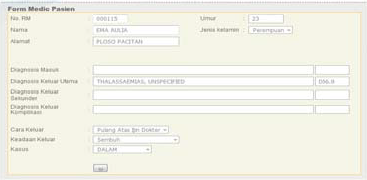
\includegraphics[width=12cm]{gambar/halaman_input_data_rekam_diagnosa.png}
		\caption{Rancangan halaman input form medis pasien. \\ Sumber: \citep{Gunawan2011sistem:11}}
		\label{Gambar:halamaninputformedispasien}
	\end{figure}
	
	\textbf{Gambar 2.29} menampilkan Rancangan halaman input form medis pasien yang berisi \emph{field} No. RM, \emph{field} nama, \emph{field} alamat, \emph{field} umur, \emph{field} jenis kelamin, \emph{field} diagnosa masuk, \emph{field} diagnosa keluar utama, \emph{field} diagnosa keluar sekunder, \emph{field} diagnosa keluar komplikasi, \emph{field} cara keluar, \emph{field} keadaan keluar, \emph{field} kasus, dan tombol ok.
	
	Dan berikut merupakan tampilan \emph{live} dari aplikasi \emph{web} jurnal kedua.
	
	\textbf{Gambar 2.30} pada halaman selanjutnya (A)menampilkan halaman \emph{login} yang berisi \emph{field} \emph{username}/\emph{email}, \emph{field} \emph{password}, tombol masuk, tombol \emph{login} dengan akun google, \emph{link} membuat akun baru, \emph{link} \emph{reset password}, dan \emph{link} bantuan. (B) menampilkan halaman registrasi yang berisi \emph{field} email, \emph{field username}, \emph{field} \emph{password}, \emph{field} nama lengkap, \emph{field} No. KTP, \emph{field} No. Telepon beserta tombol ceklis. Dan (C) menampilkan menu utama aplikasi yang berisi menu daftar \emph{online} rawat jalan, menu profil, menu rawat inap, menu dokter, menu rawat jalan, menu penunjang, menu galeri, menu daftar \emph{online}, menu efek samping obat, menu info kamar, menu telepon, menu akun, dan menu lainnya.
	
	\begin{figure}[H]
		\centering
		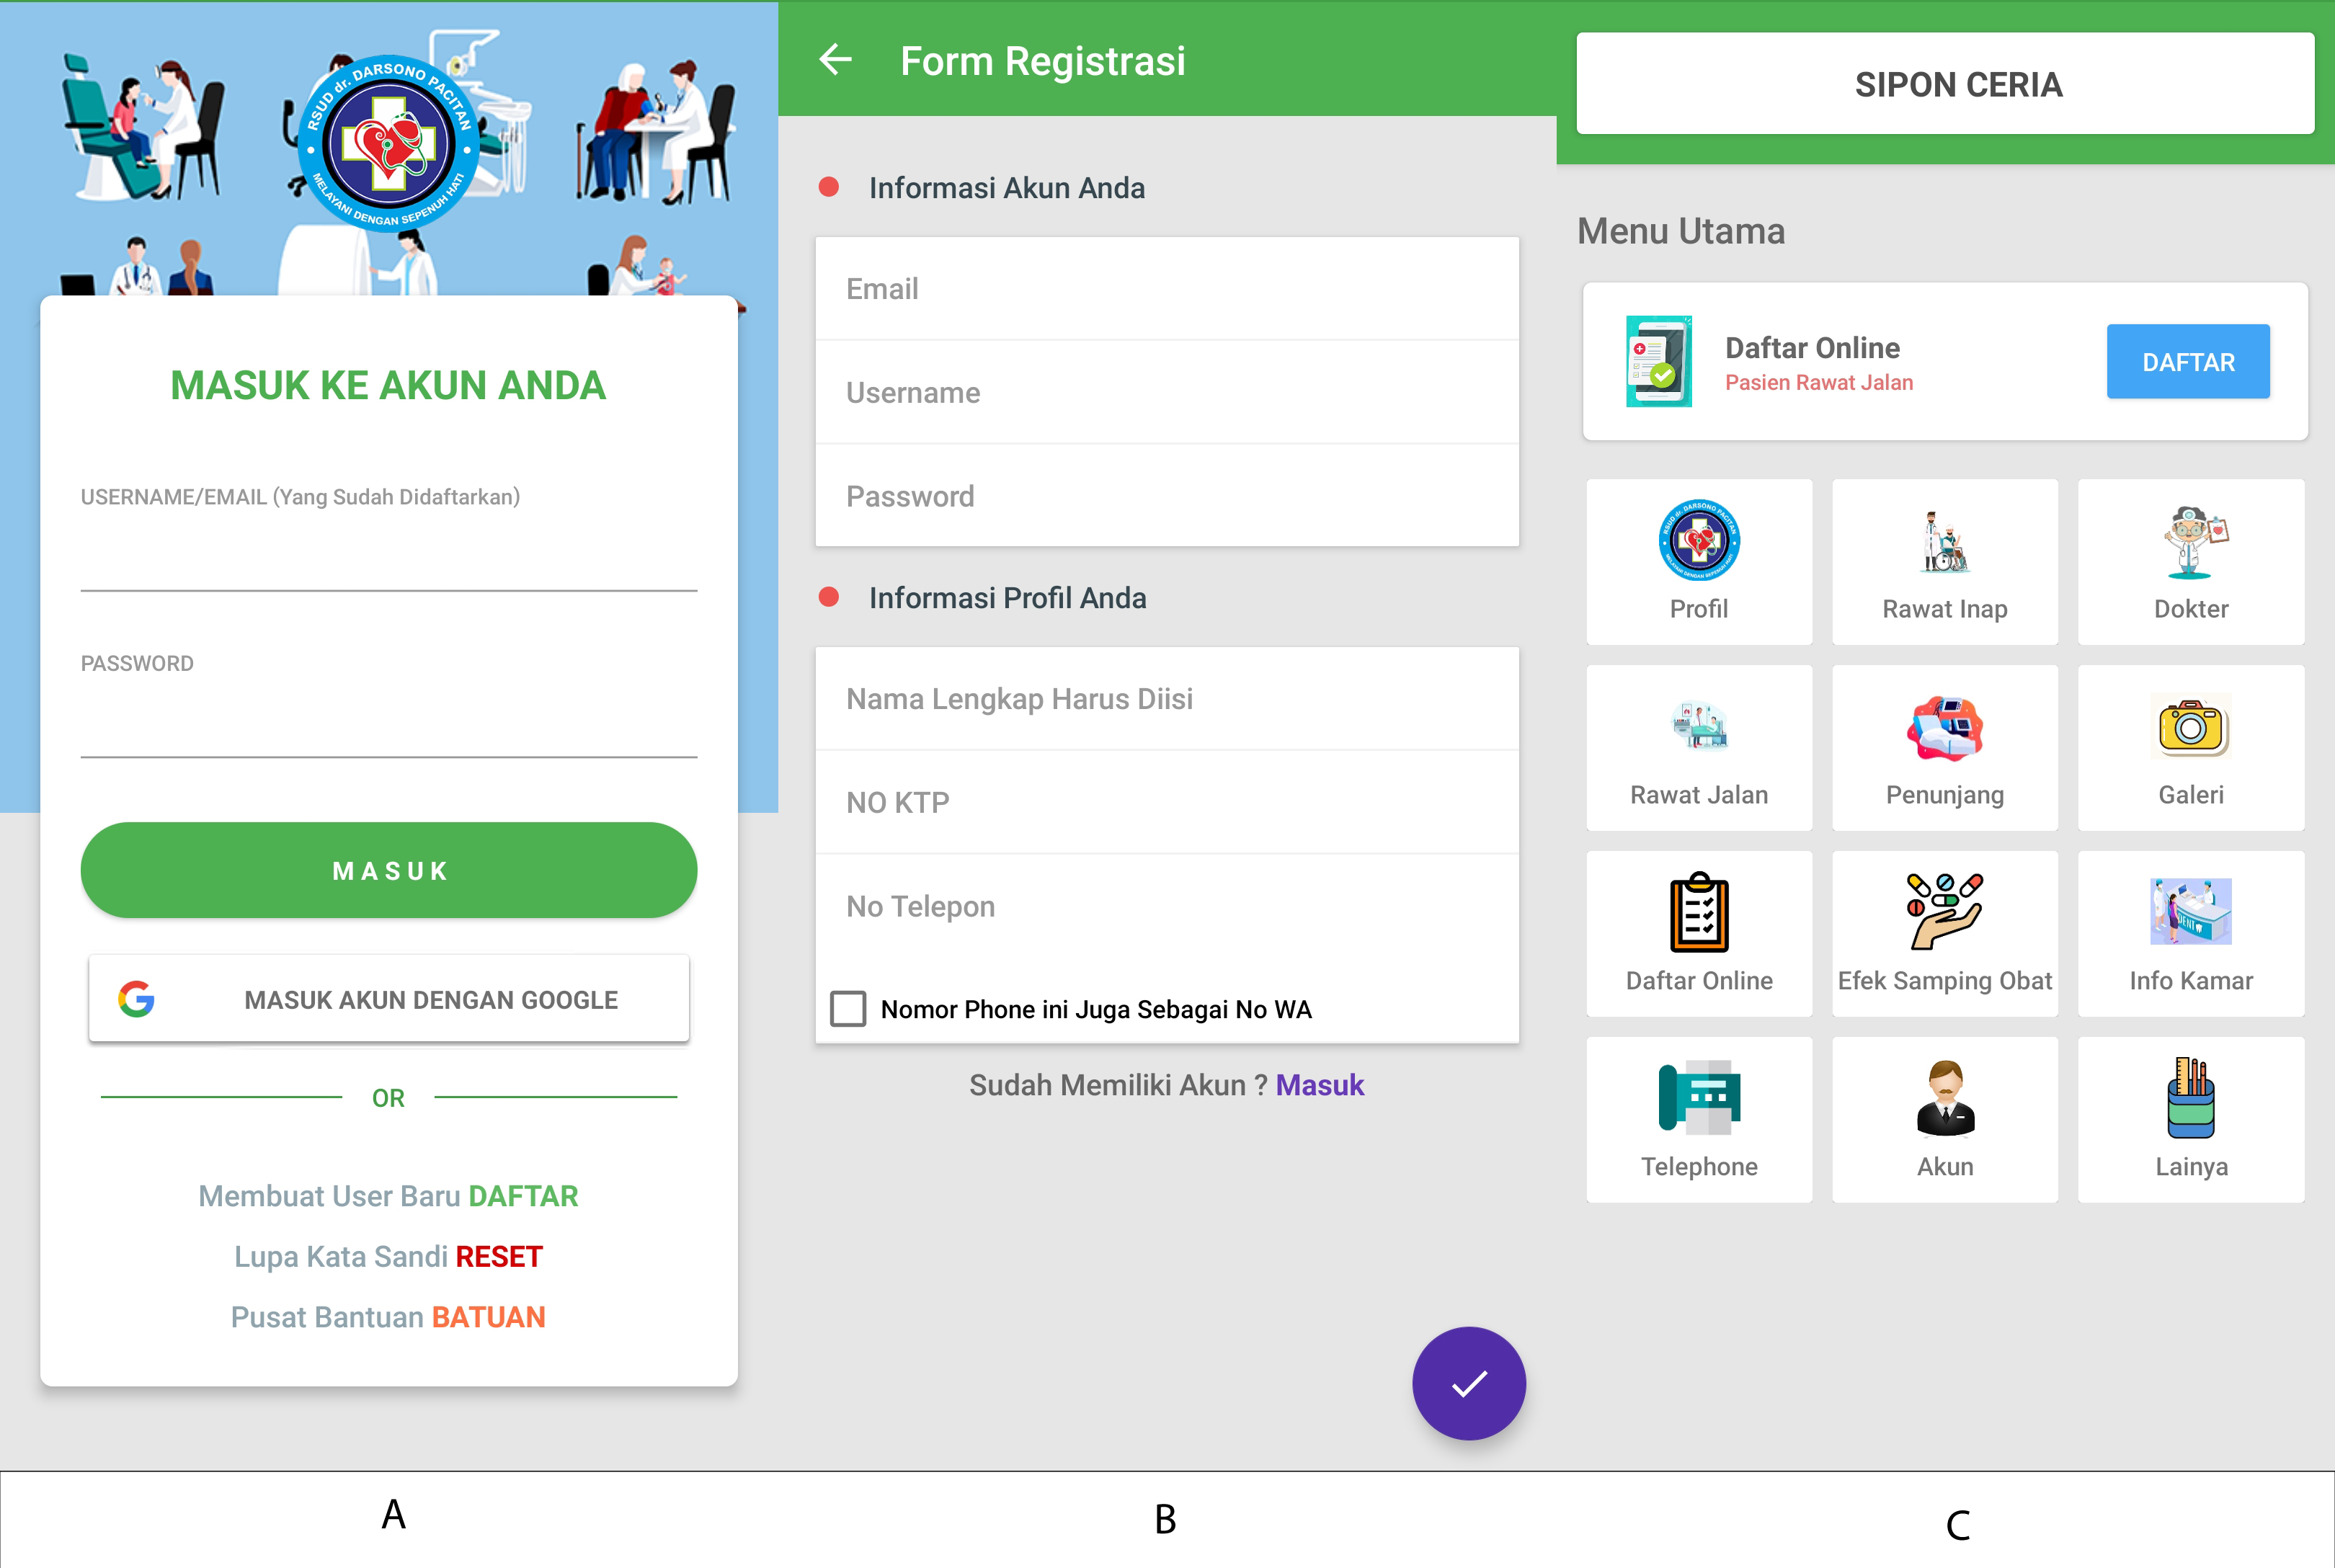
\includegraphics[width=12cm]{gambar/1.jpg}
		\caption{(A) Halaman login. (B)Halaman registrasi. (C)Halaman awal. \\ Sumber: Aplikasi android SIPON CERIA}
		\label{Gambar:halamanlive0jurnal2}
	\end{figure}
	
	\textbf{Gambar 2.31} pada halaman selanjutnya (A)menampilkan halaman input data pasien yang berisi \emph{field} hubungan dengan keluarga, \emph{field} No. RM, \emph{field} tanggal lahir pasien, \emph{field} No. Telepon, \emph{field} email, dan \emph{field} No. KTP. (B) menampilkan halaman bukti pendaftaran pasien. Dan (C) menampilkan halaman riwayat daftar \emph{online}.
	
	\begin{figure}[H]
		\centering
		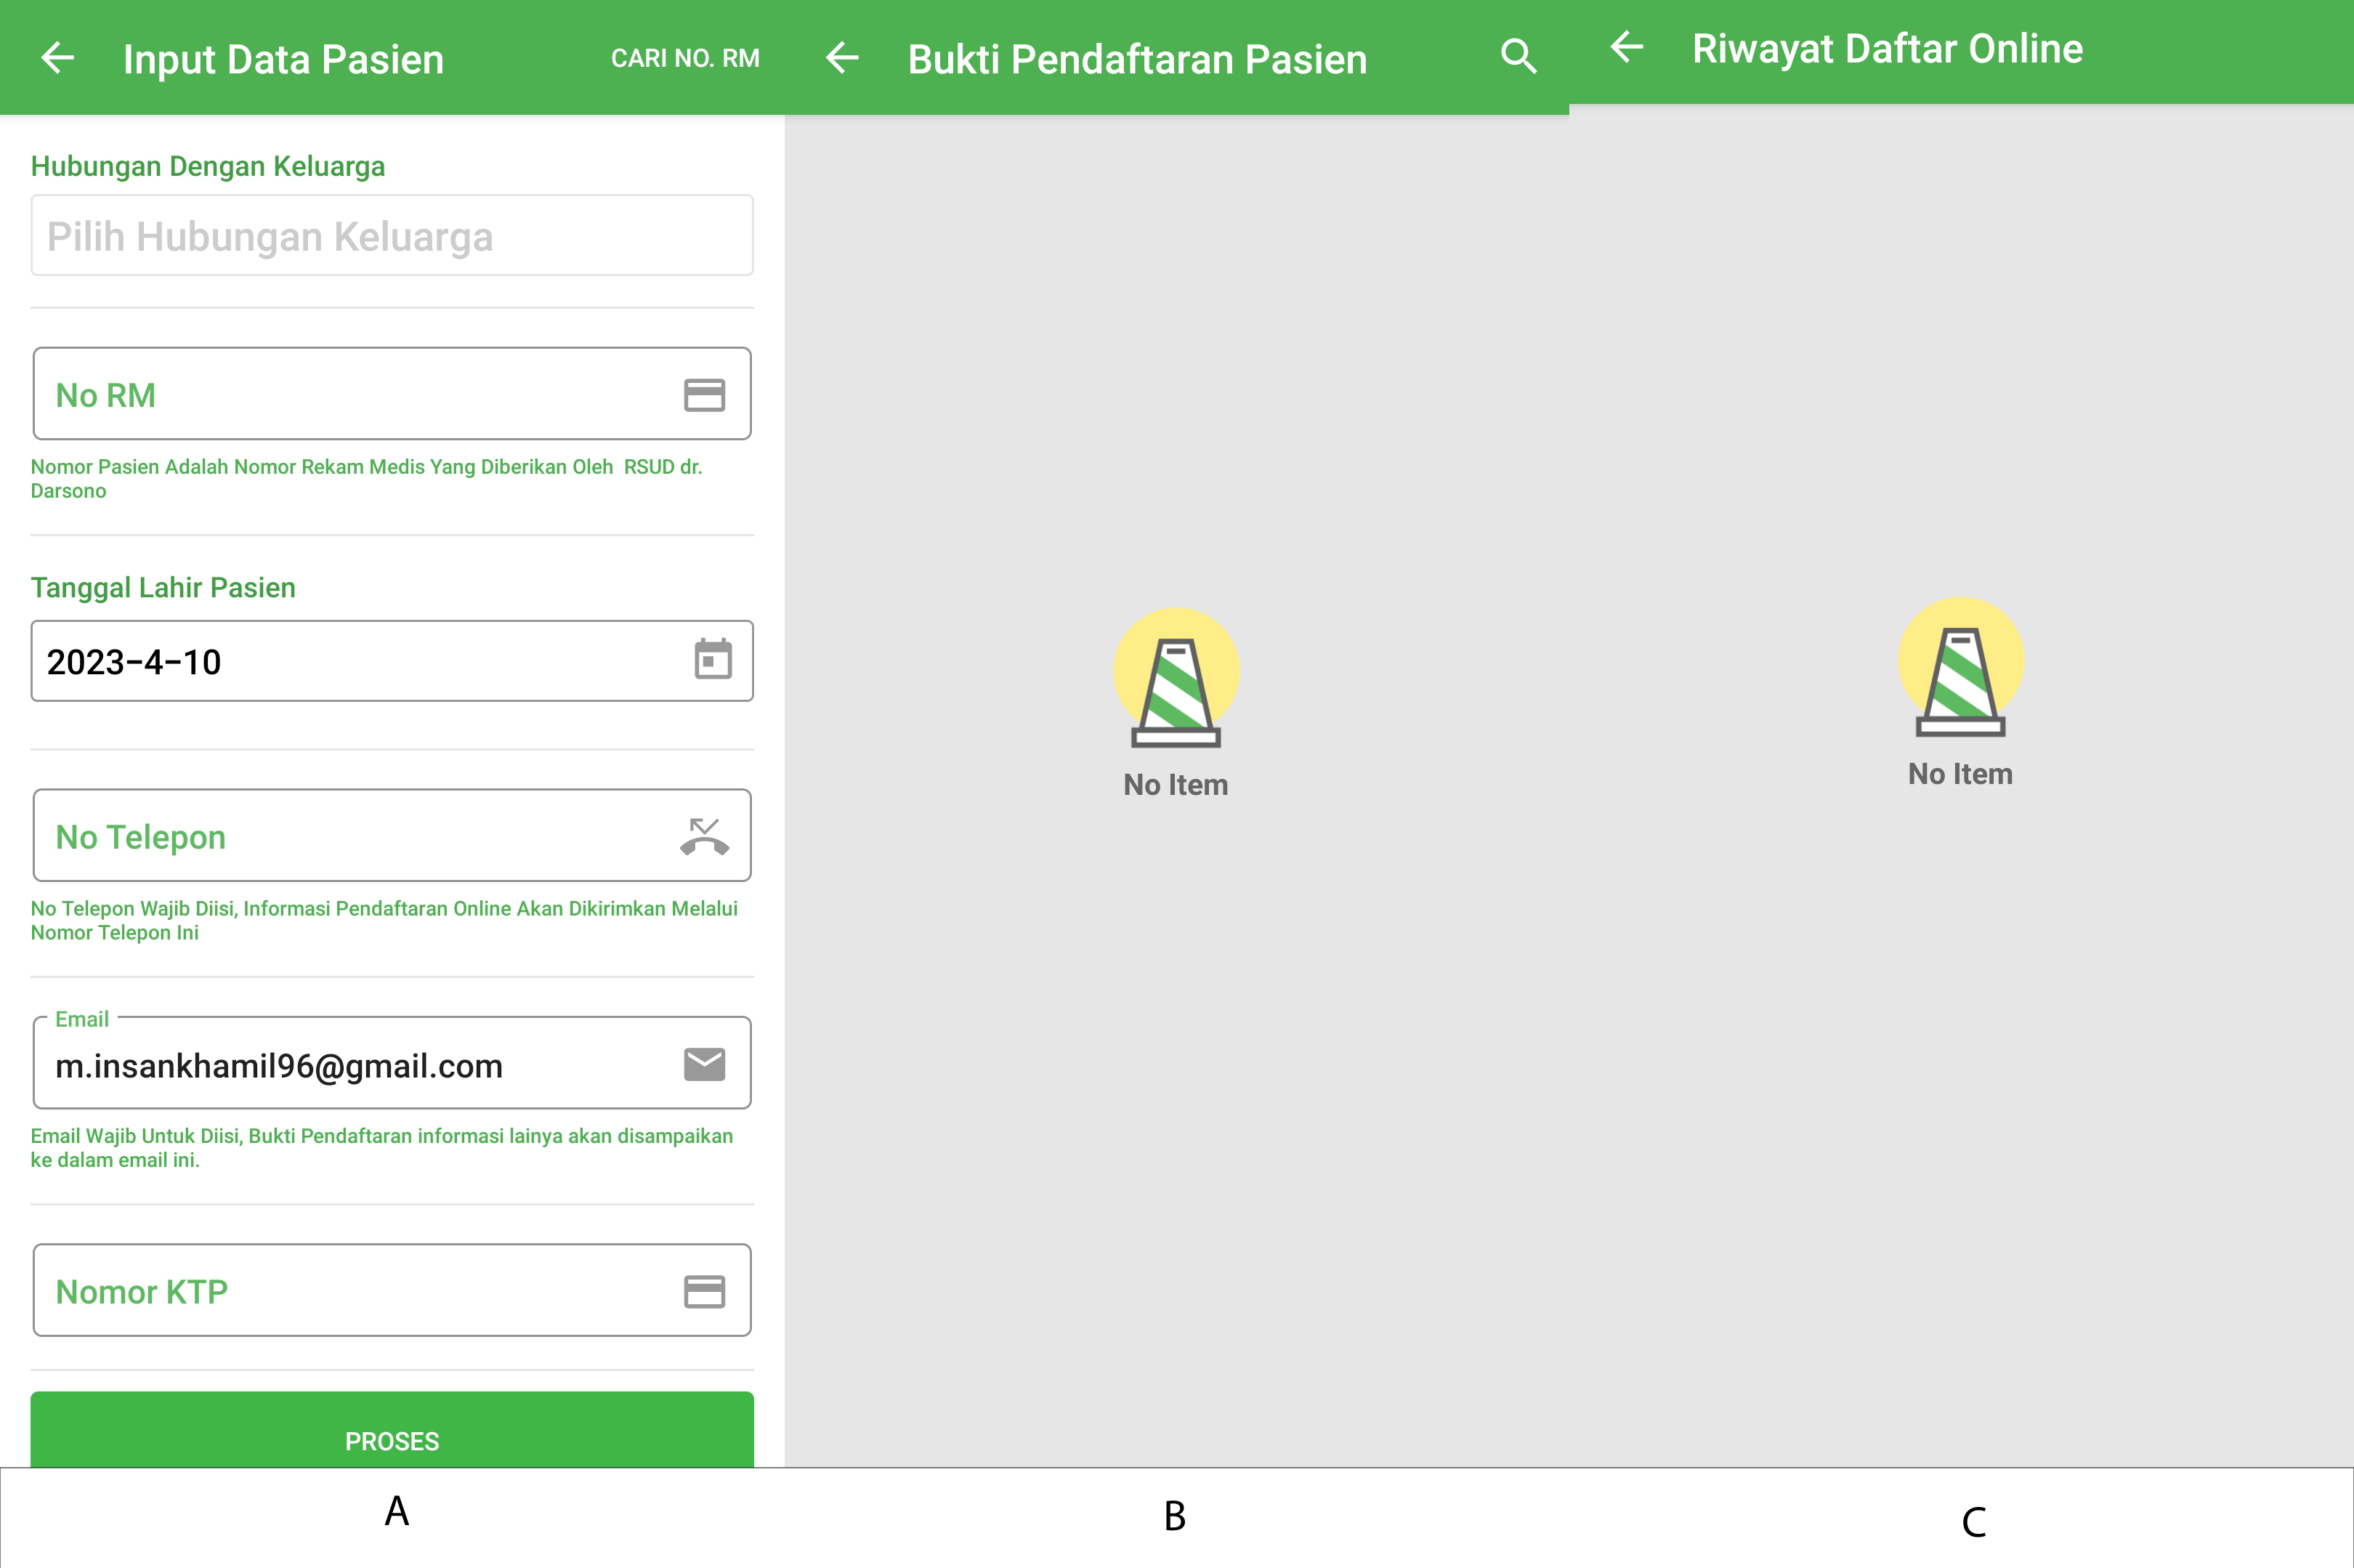
\includegraphics[width=12cm]{gambar/2.jpg}
		\caption{(A) Halaman \emph{input} data pasien. (B) Halaman bukti pendaftaran pasien. (C) Halaman riwayat daftar pasien. \\ Sumber: Aplikasi android SIPON CERIA}
		\label{Gambar:halamanlive1jurnal2}
	\end{figure}
	
	
	\begin{figure}[H]
		\centering
		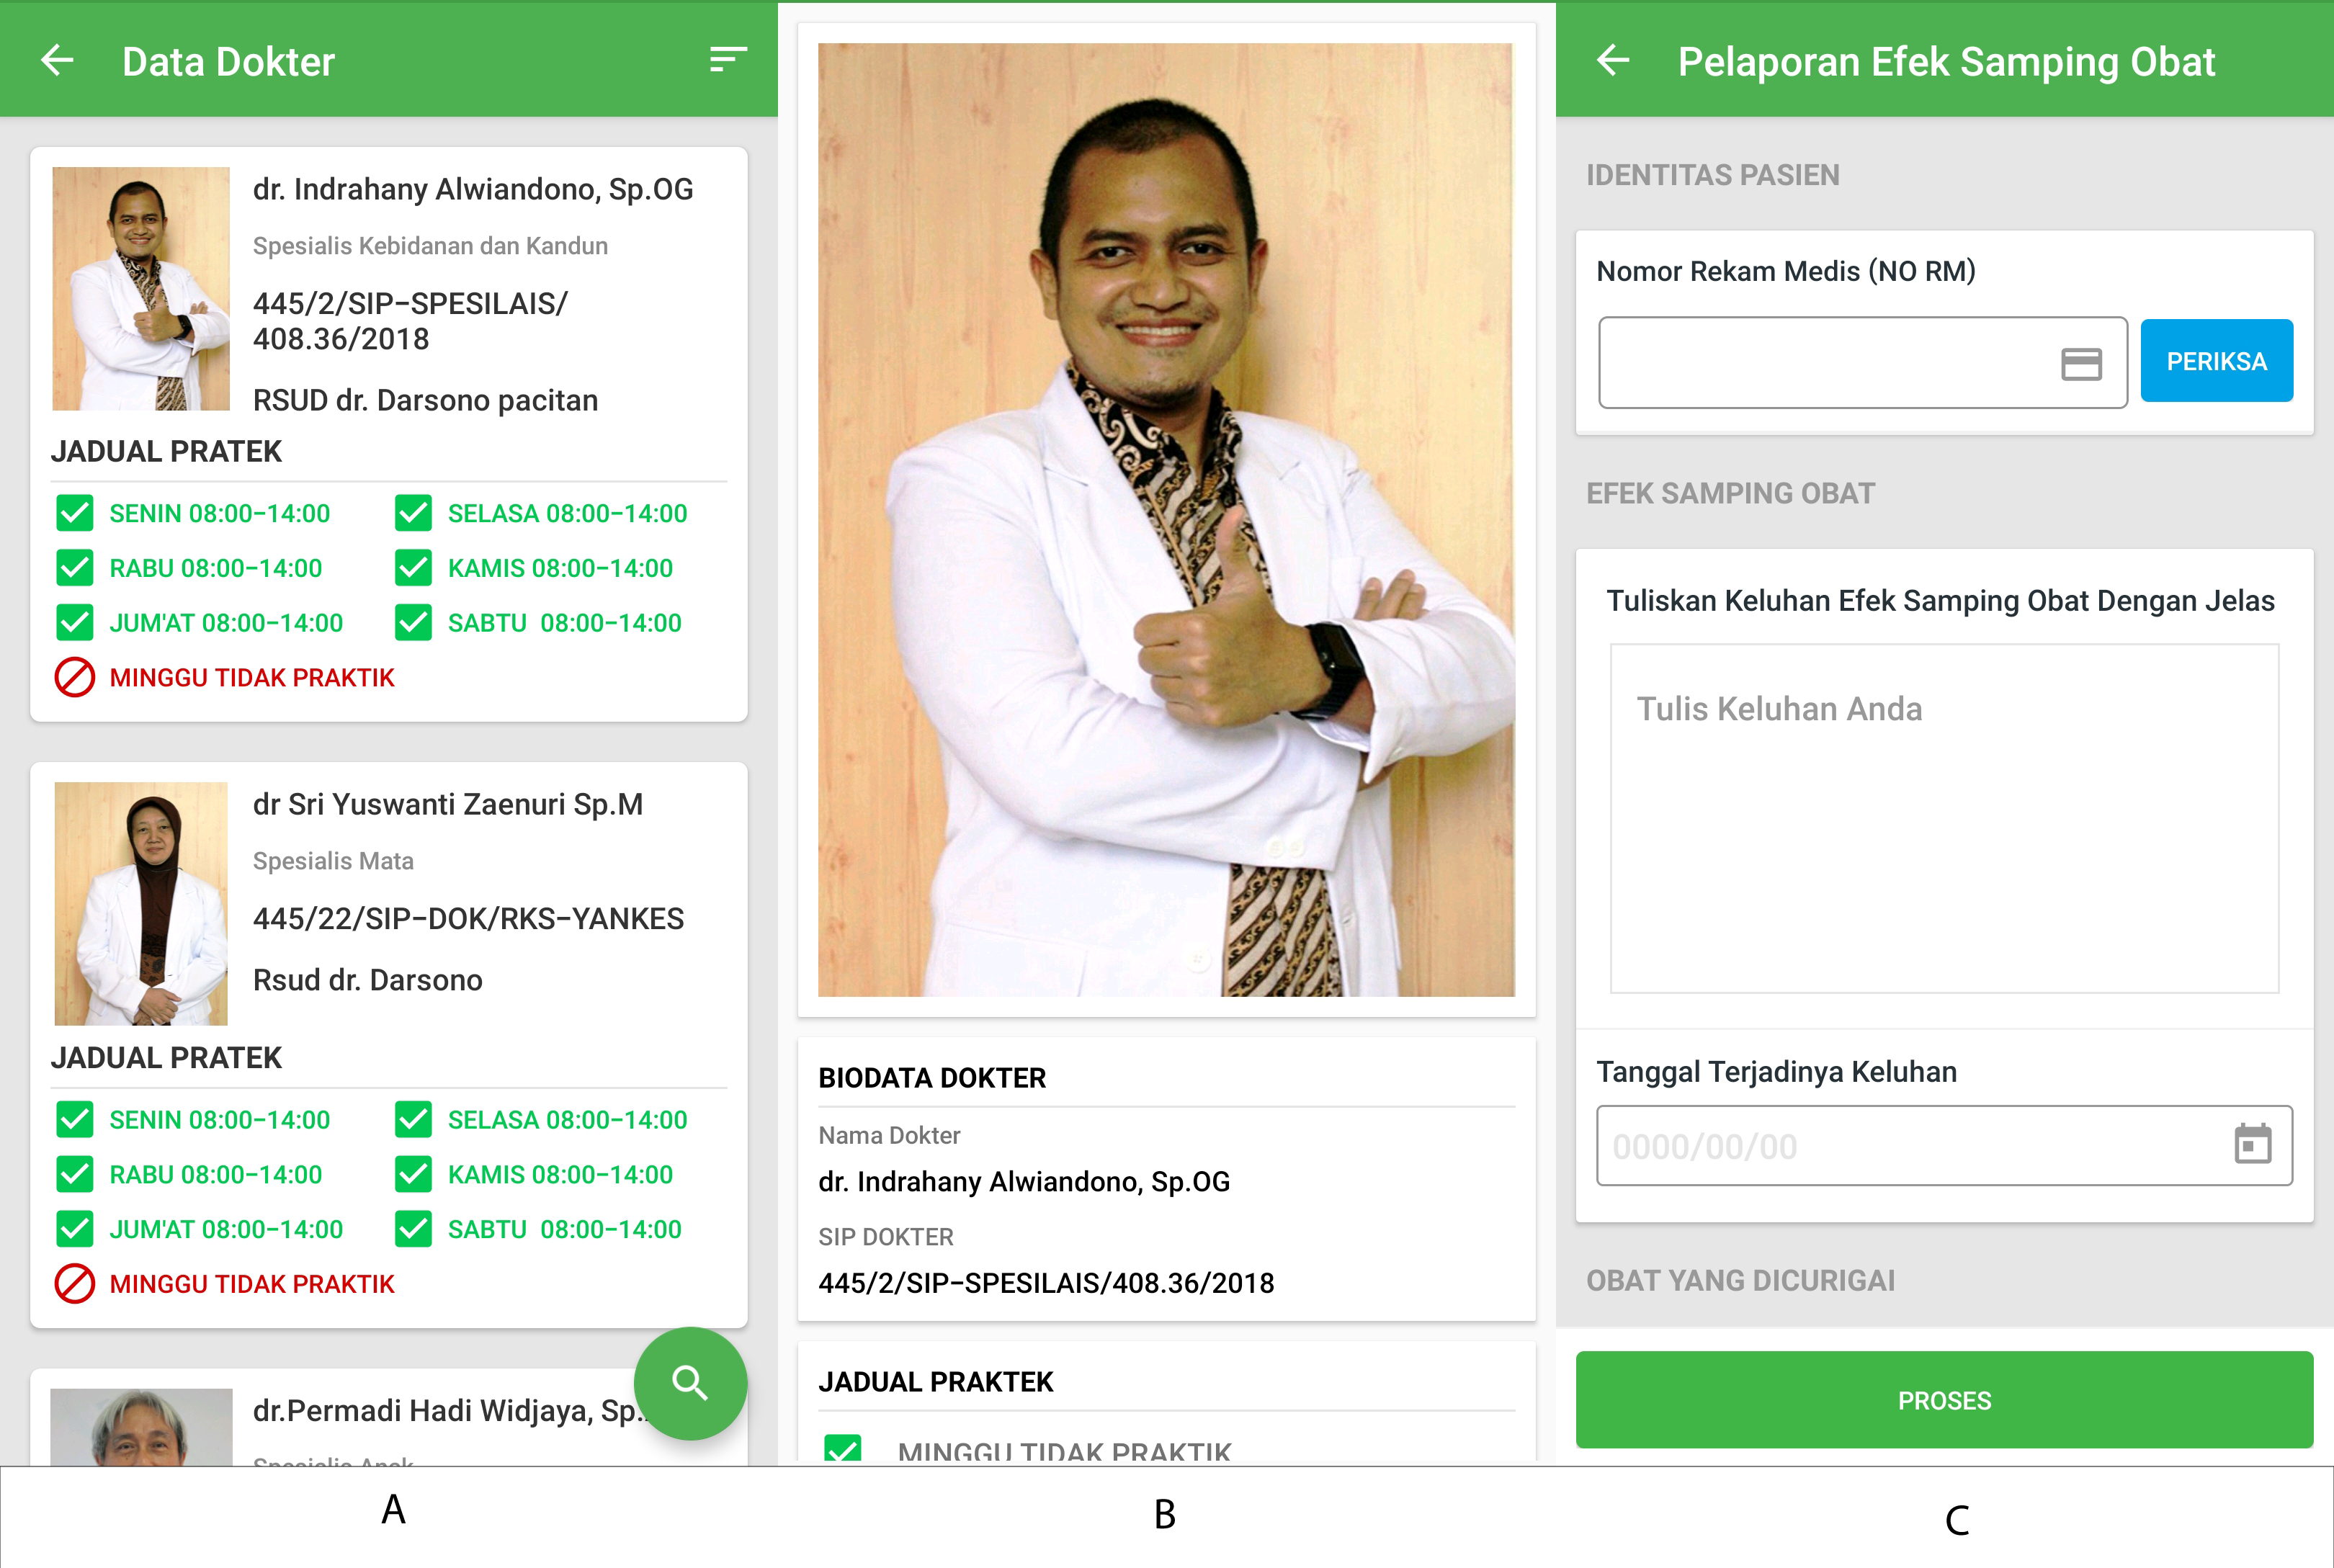
\includegraphics[width=12cm]{gambar/3.jpg}
		\caption{(A) Halaman \emph{list} dokter. (B) Halaman detail data dokter. (C) Halaman menu pelaporan efek samping obat. \\ Sumber: Aplikasi android SIPON CERIA}
		\label{Gambar:halamanlive2jurnal2}
	\end{figure}
	
	\textbf{Gambar 2.32} (A)menampilkan halaman \emph{list} dokter yang berisi \emph{list} dokter yang tersedia lengkap dengan foto, nama, spesialis bidang, dan jadwal praktek. (B) menampilkan halaman detail data dokter yang berisi biodata dokter lengkap. Dan (C) menampilkan halaman menu pelaporan efek samping obat yang berisi \emph{field} No. RM, \emph{field} keluhan efek samping, \emph{field} tanggal terjadinya keluhan dan \emph{field} nama obat yang dicurigai.
	
	\textbf{Gambar 2.33} (A)menampilkan halaman menu rawat jalan yang berisi \emph{list} poliklinik beserta jadwal pelayanan. (B) menampilkan halaman \emph{list} data dokter yang berkaitan dengan poliklinik yang dipilih. Dan (C) menampilkan halaman \emph{list} fasilitas poliklinik yang dipilih.
	
	\begin{figure}[H]
		\centering
		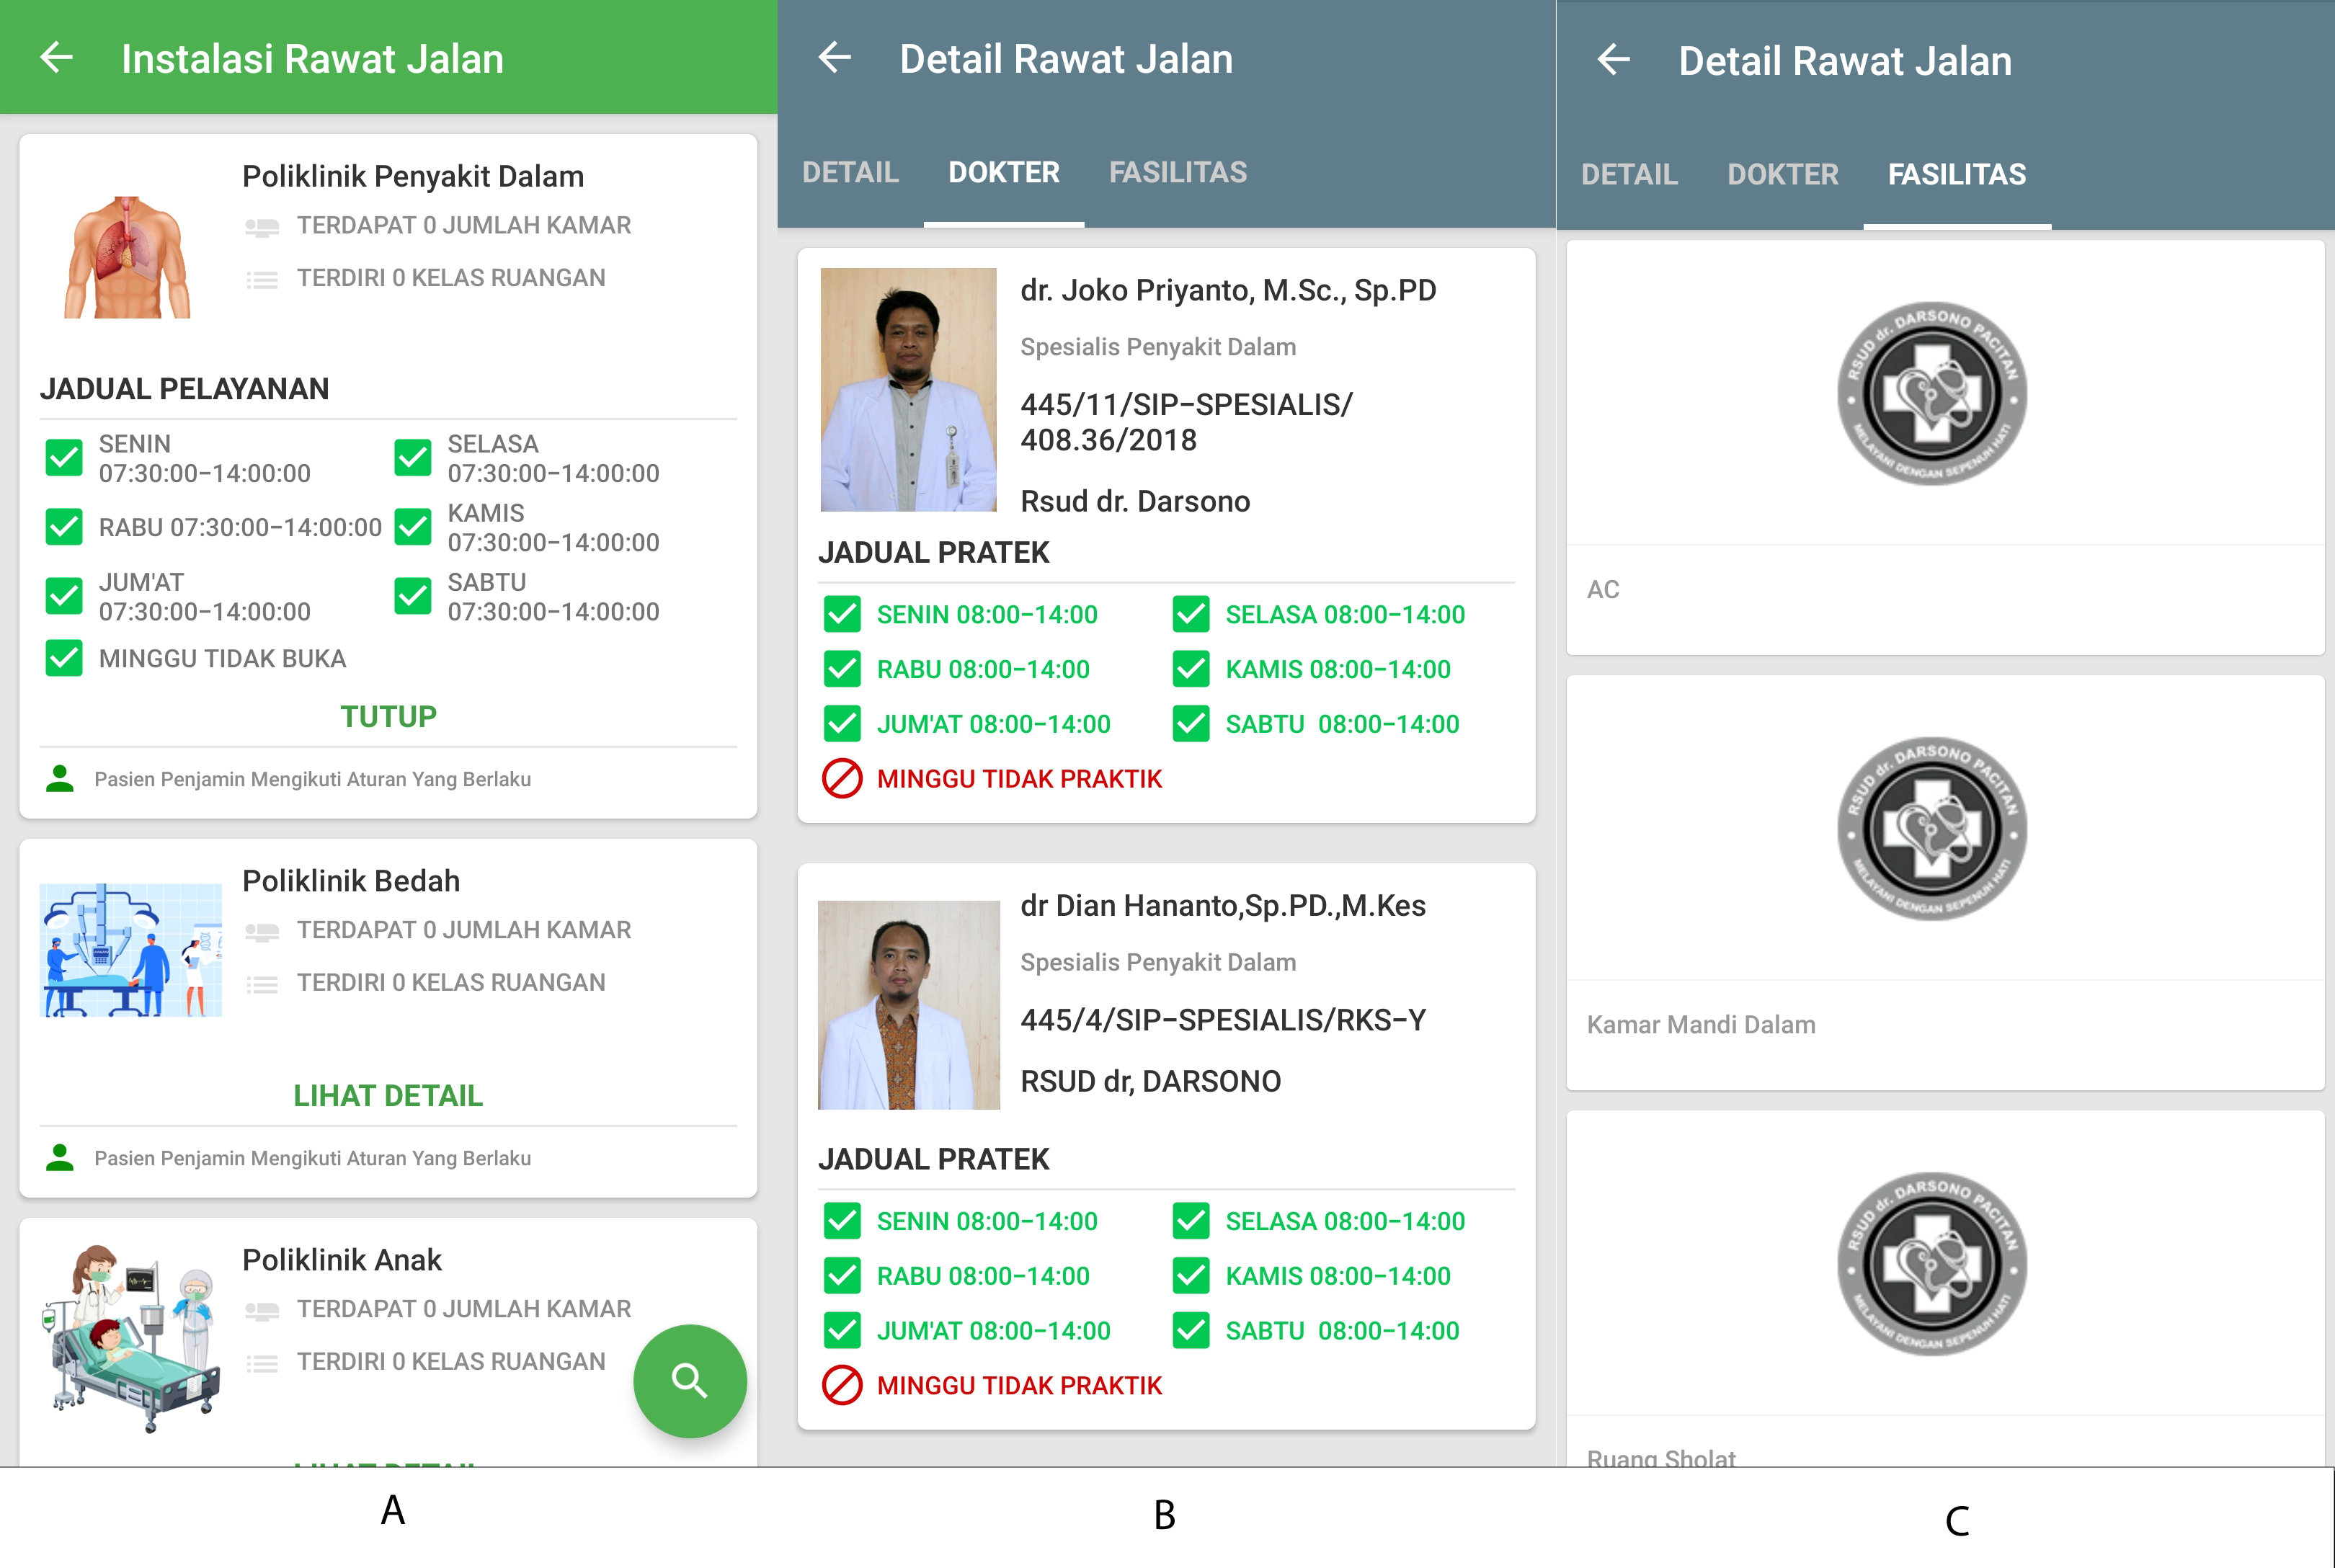
\includegraphics[width=12cm]{gambar/4.jpg}
		\caption{(A) Halaman menu rawat jalan. (B) Halaman detail rawat jalan \emph{list} dokter. (C) Halaman detail rawat jalan \emph{list} fasilitas. \\ Sumber: Aplikasi android SIPON CERIA}
		\label{Gambar:halamanlive3jurnal2}
	\end{figure}
	
	\begin{figure}[H]
		\centering
		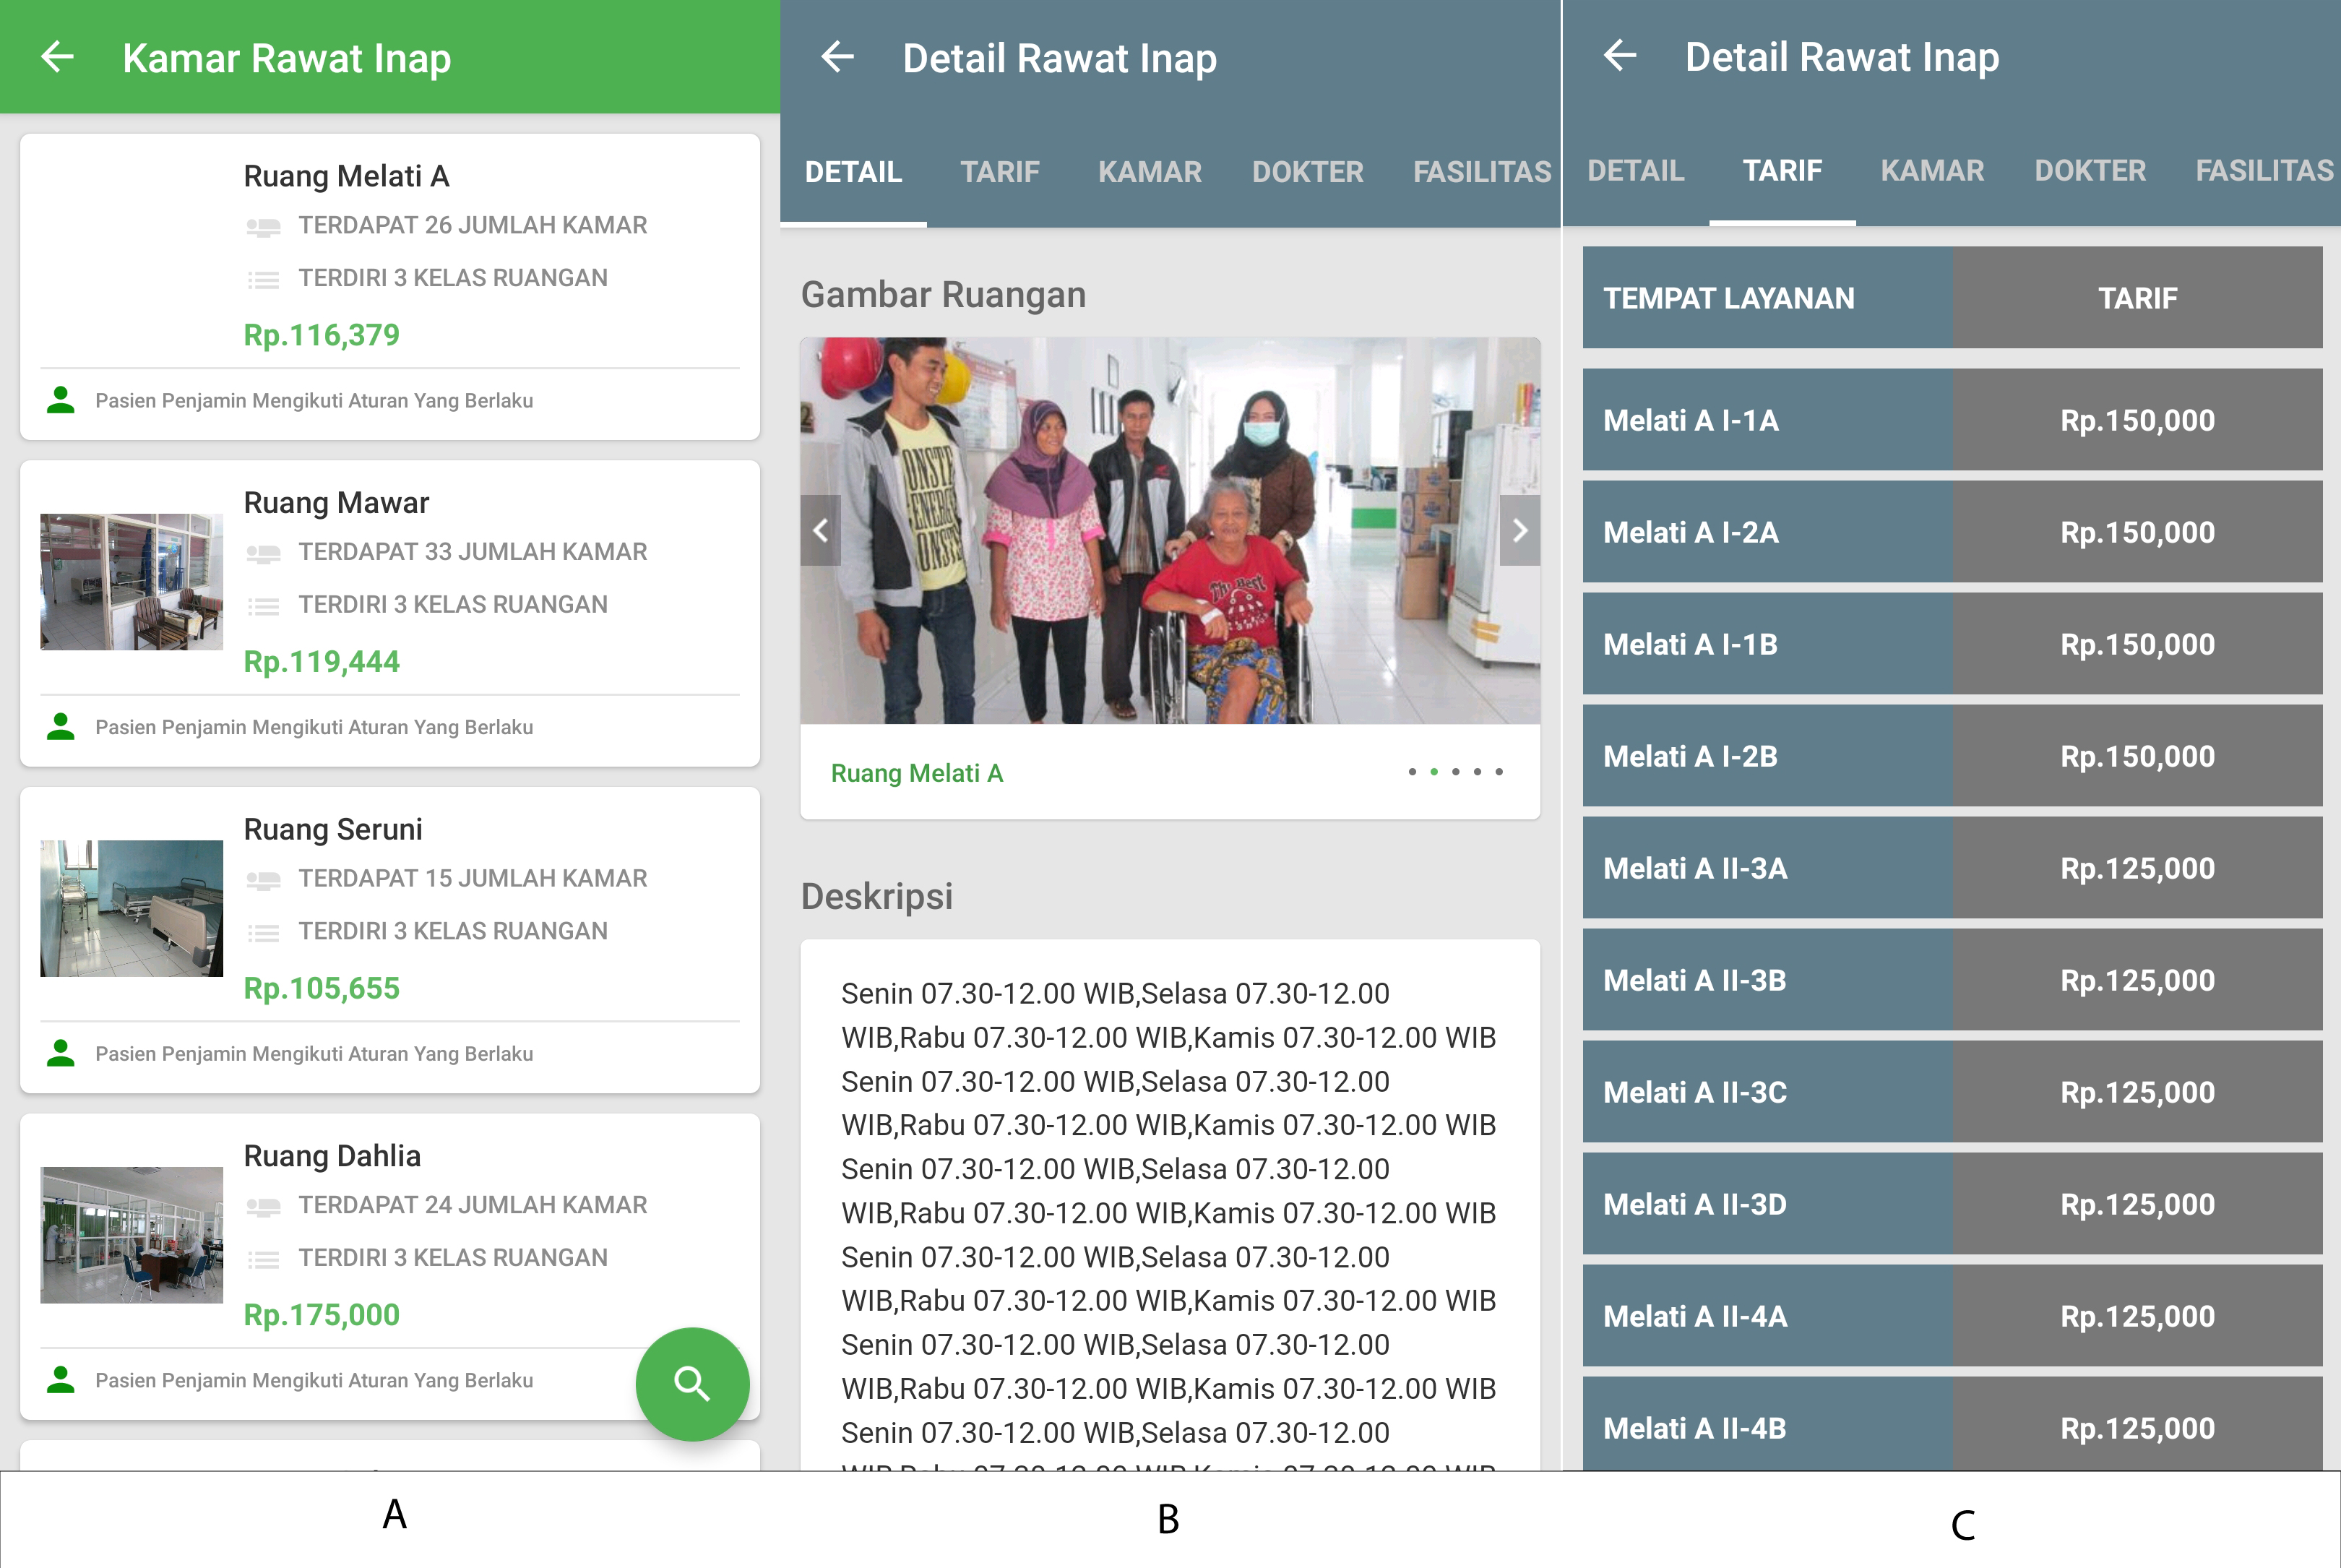
\includegraphics[width=12cm]{gambar/5.jpg}
		\caption{(A) Halaman menu rawat inap. (B) Halaman detail rawat inap detail. (C) Halaman detail rawat inap \emph{list} tarif. \\ Sumber: Aplikasi android SIPON CERIA}
		\label{Gambar:halamanlive4jurnal2}
	\end{figure}
	
	\textbf{Gambar 2.34} (A)menampilkan halaman menu rawat inap yang berisi \emph{list} ruang rawat inap beserta foto ruangan dan harganya. (B) menampilkan halaman detail ruang rawat inap yang dipilih. Dan (C) menampilkan halaman \emph{list} harga ruangan rawat inap yang dipilih sesuai kelas.
	
	\textbf{Gambar 2.35} pada halaman selanjutnya (A)menampilkan halaman \emph{list} ruang rawat inap berdasarkan kelas, detail dan harganya. (B) menampilkan halaman \emph{list} dokter yang berkaitan dengan rawat inap . Dan (C) menampilkan halaman \emph{list} fasilitas ruangan rawat inap yang dipilih.
	
	\begin{figure}[H]
		\centering
		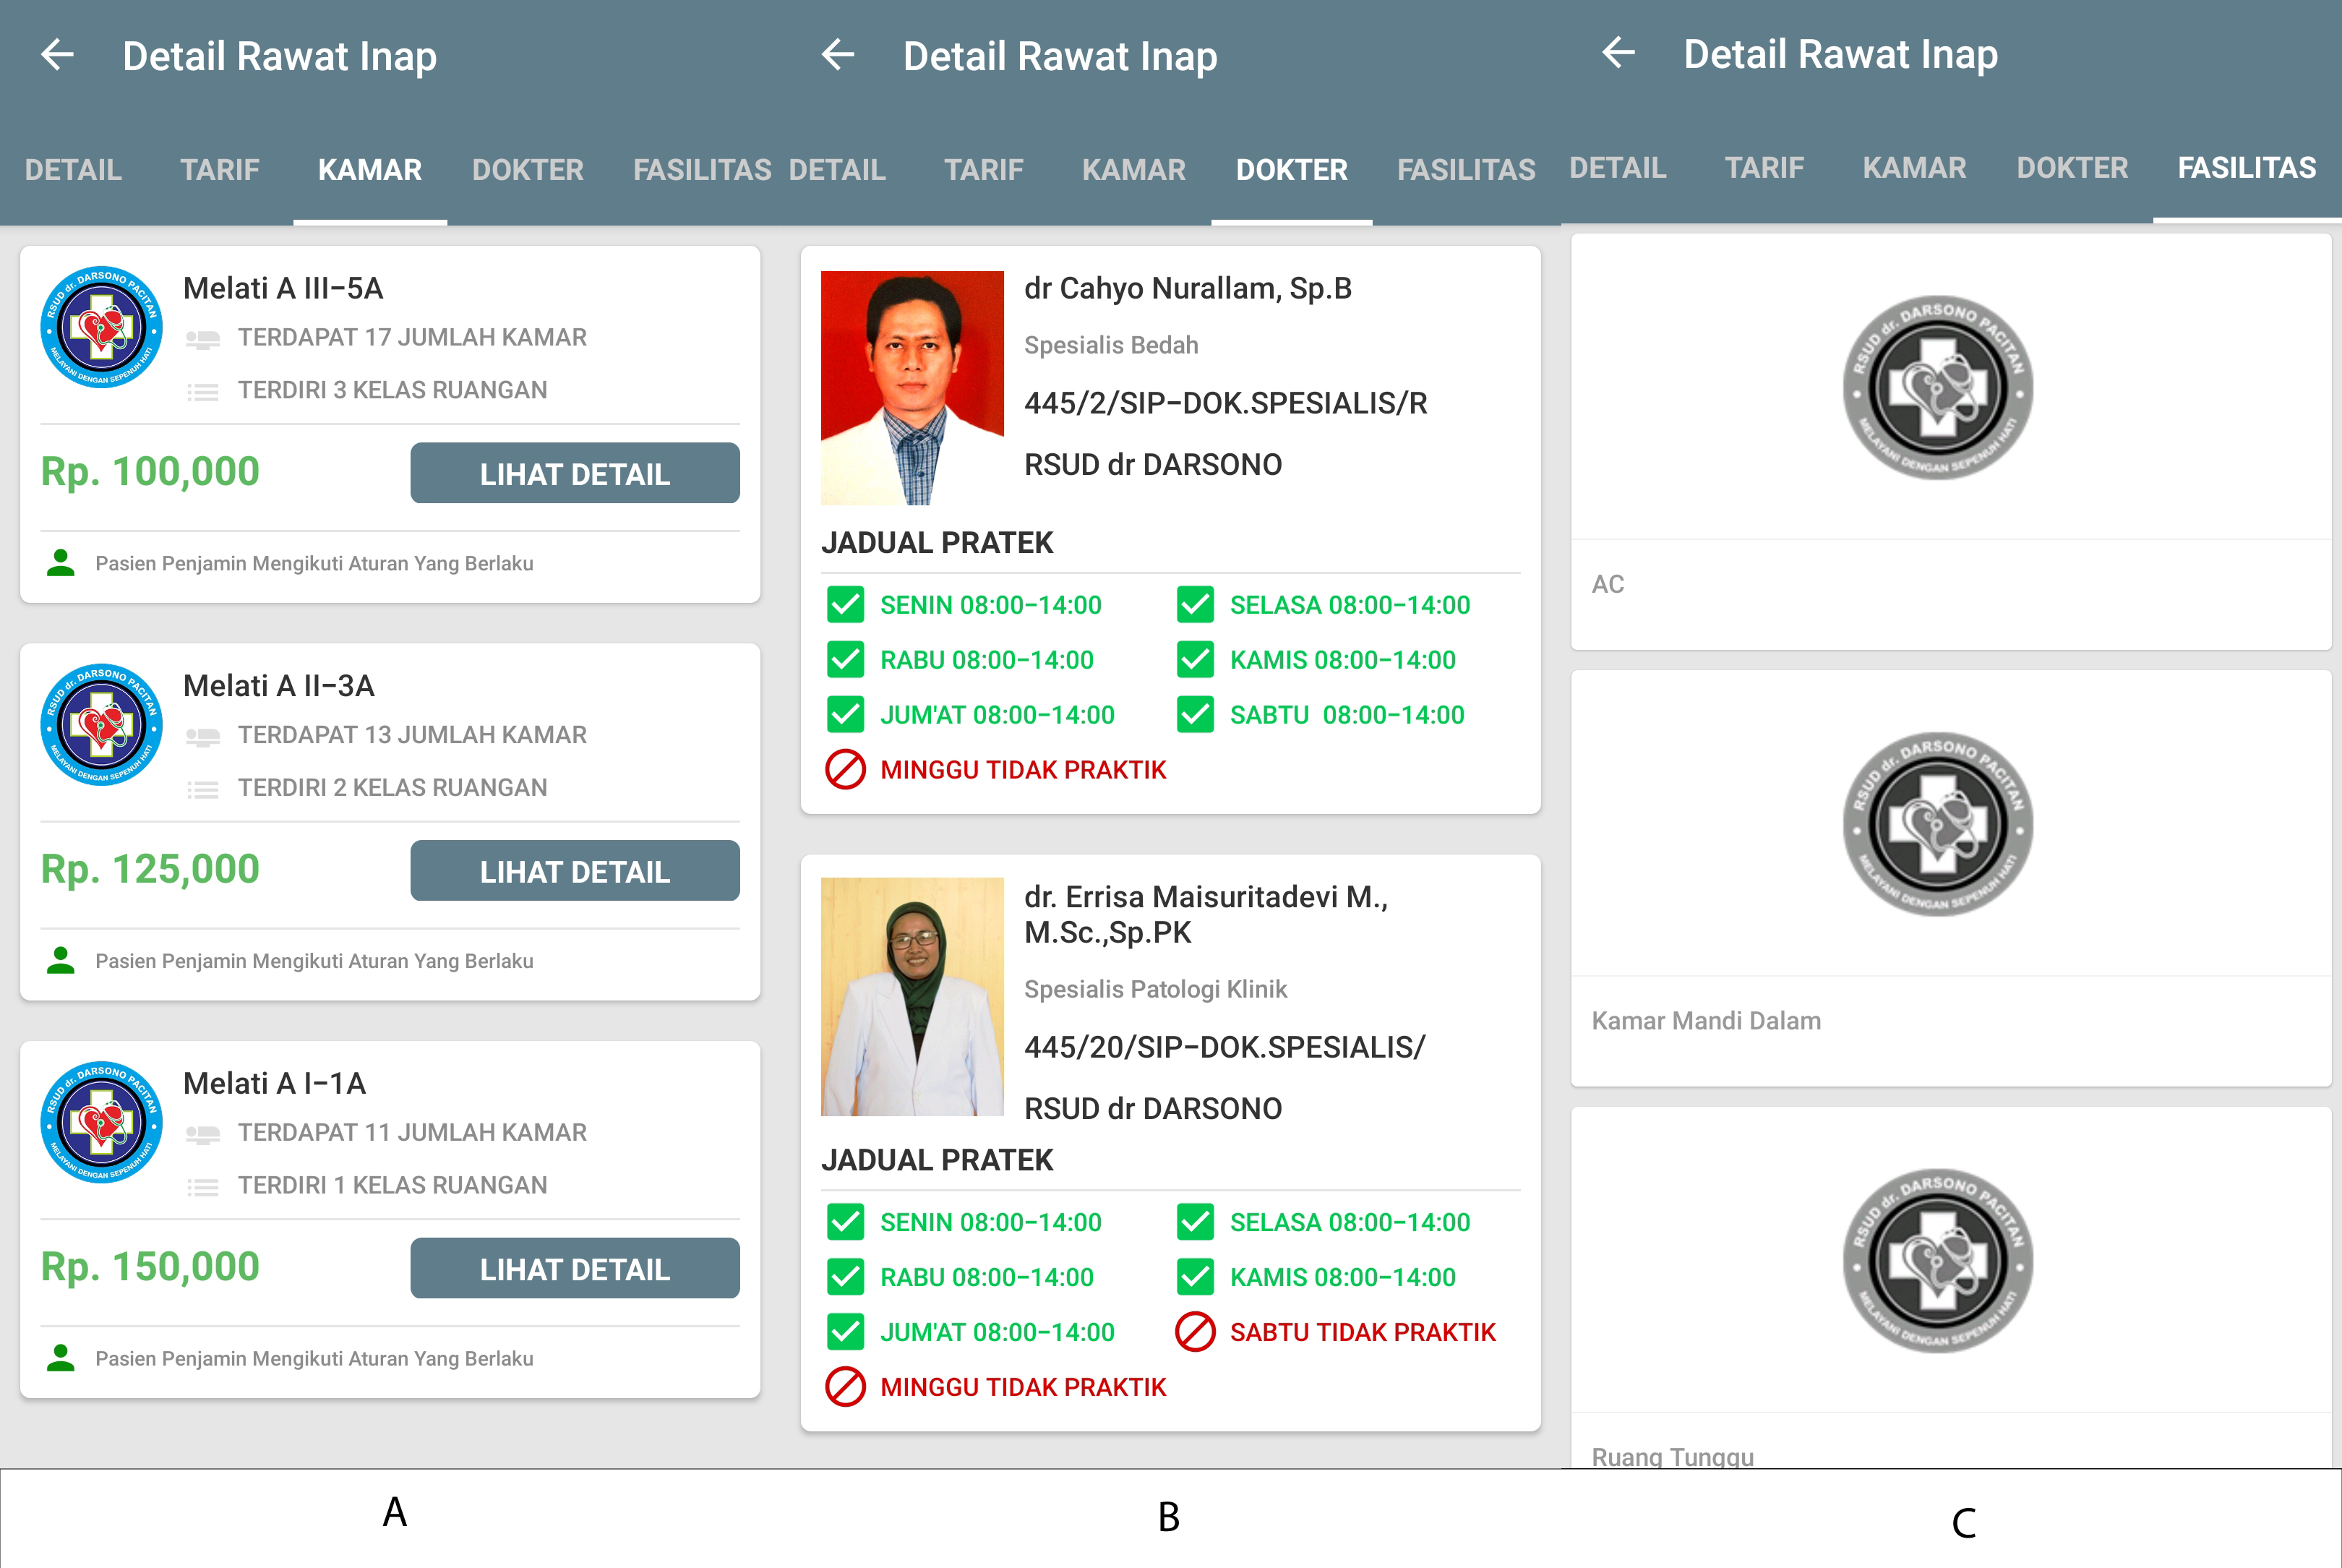
\includegraphics[width=12cm]{gambar/6.jpg}
		\caption{(A) Halaman detail rawat inap \emph{list} kamar. (B) Halaman detail rawat inap \emph{list} dokter. (C) Halaman \emph{list} fasilitas ruangan rawat inap. \\ Sumber: Aplikasi android SIPON CERIA}
		\label{Gambar:halamanlive5jurnal2}
	\end{figure}
	
	\item UI/UX pada jurnal ketiga
	
	Berikut di bawah ini merupakan UI/UX yang ditampilkan didalam jurnal ketiga. Pada jurnal ini hanya ditampilkan satu dari 12 UI/UX, yaitu halaman membuat reservasi.
	
	\textbf{Gambar 2.36} pada halaman selanjutnya menampilkan Rancangan halaman membuat reservasi berobat yang berisi \emph{field} nama pasien, \emph{field} jenis kelamin, \emph{field} tempat lahir, \emph{field} tanggal lahir, \emph{field} umur, \emph{field} status pernikahan, \emph{field} tanggal reservasi, \emph{field} pekerjaan, \emph{field} alamat lengkap, \emph{field} kecamatan.
	
	\begin{figure}[H]
		\centering
		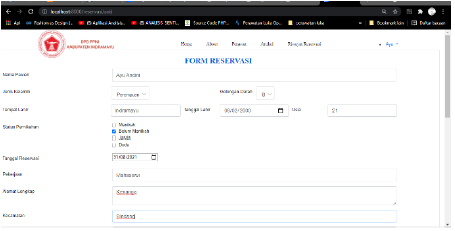
\includegraphics[width=12cm]{gambar/halaman_membuat_reservasi.png}
		\caption{Rancangan halaman membuat reservasi \emph{online} \\ Sumber: \cite{Carminah2021aplikasi:12}}
		\label{Gambar:halamanmembuatreservasionline}
	\end{figure}
	
	Dan pada jurnal ketiga tidak ditemukan \emph{website live}-nya.
	
\end{enumerate}

\subsection{Kesimpulan Studi Banding}

Tabel di bawah ini merupakan tabel fitur sistem informasi rumah sakit berdasarkan 3 jurnal yang telah peneliti sebutkan sebelumnya.

\begin{table}[H]
	\centering
	\caption{Tabel fitur sistem informasi rumah sakit}
	\label{tabel_input}
	\begin{tabular}{|c|m{7cm}|c|c|c|}
		\hline
		\textbf{No} & \textbf{Fitur} & \textbf{Jurnal 1} & \textbf{Jurnal 2} & \textbf{Jurnal 3} \\
		\hline
		
		& 
		\textbf{Dari sisi pasien} &
		& &\\
		\hline 
		
		1& 
		Melihat data dokter                      
		(pasien dapat melihat detail data dokter) &
		\tickYes& &\\
		\hline
		
		2& 
		Melihat jadwal dokter
		(pasien dapat melihat jadwal dokter) &
		\tickYes& &\\
		\hline
		
		3 & 
		Melihat jumlah pasien yang telah nendaftar berobat
		(pasien dapat melihat pasien lain yang telah daftar berobat) &
		\tickYes& &\\
		\hline
		
	\end{tabular}
\end{table}

\begin{table}[H]
	\centering
	\caption{Fitur sistem informasi rumah sakit - lanjutan 1}
	\label{tabel_input}
	\begin{tabular}{|c|m{7cm}|c|c|c|}
		\hline
		\textbf{No} & \textbf{Fitur} & \textbf{Jurnal 1} & \textbf{Jurnal 2} & \textbf{Jurnal 3} \\
		\hline
		
		& 
		\textbf{Dari sisi pasien} &
		& &\\
		\hline
		
		4 & 
		Pasien bisa mengelola akun sendiri
		(pasien dapat membuat dan merubah akun \emph{online} secara mandiri) &
		& \tickYes &\\
		\hline
		
		5 & 
		Melakukan pendaftaran berobat secara \emph{online}
		(pasien dapat melakukan pendaftaran berobat \emph{online}) &
		\tickYes& \tickYes &\\
		\hline
		
		6 & 
		Melihat notifikasi sms nomor antrian berobat
		(pasien mendapatkan sms dan dapat mengetahui nomor antrian berobatnya) &
		\tickYes& &\\
		\hline
		
		7 & 
		Melihat status berobat (pasien dapat melihat status berobat mereka yaitu sudah diverifikasi, belum diverifikasi, \emph{cancel})&
		\tickYes & &\\
		\hline
		
		& 
		\textbf{Dari sisi pegawai rumah sakit} &
		& &\\
		\hline
		
		8 & 
		Mengelola akun pasien (pegawai rumah sakit dapat menambah, menghapus, merubah akun pasien) &
		\tickYes & \tickYes &\\
		\hline
		
		9 & 
		Mengelola akun pegawai rumah sakit (pegawai rumah sakit dapat menambah, menghapus, merubah akun pegawai rumah sakit) &
		\tickYes & & \tickYes \\
		\hline
		
	\end{tabular}
\end{table}

\begin{table}[H]
	\centering
	\caption{Tabel fitur sistem informasi rumah sakit - lanjutan 2}
	\label{tabel_input}
	\begin{tabular}{|c|m{7cm}|c|c|c|}
		\hline
		\textbf{No} & \textbf{Fitur} & \textbf{Jurnal 1} & \textbf{Jurnal 2} & \textbf{Jurnal 3} \\
		\hline
		
		& 
		\textbf{Dari sisi pegawai rumah sakit} &
		& &\\
		\hline
		
		10 & 
		Mendaftarkan pasien berobat (pegawai rumah sakit dapat mendaftarkan pasien berobat secara \emph{offline} di tempat) &
		& \tickYes &\\
		\hline
		
		11 & 
		Mengelola status pasien berobat (pegawai rumah sakit dapat memberikan status verifikasi atau \emph{cancel}) &
		\tickYes& & \tickYes \\
		\hline
		
		12 & 
		Membuat data rekam medis pasien (pegawai rumah sakit dapat membuat laporan data rekam medis pasien yang telah berobat) &
		& \tickYes & \tickYes \\
		\hline
		
		13 & 
		Mengelola jadwal dokter (pegawai rumah sakit dapat menambah dan merubah jadwal praktik dokter sesuai kebutuhan) &
		\tickYes& &\\
		\hline
		
		14 & 
		Mengelola jadwal dokter (pegawai rumah sakit dapat menambah dan merubah jadwal praktik dokter sesuai kebutuhan) &
		\tickYes& &\\
		\hline
		
		15 & 
		Mengelola inventaris rumah sakit (pegawai rumah sakit dapat menambah \emph{item}, menghapus \emph{item}, merubah \emph{item}, mengurangi kuantitas \emph{item}, menambah kuantitas \emph{item} inventaris rumah sakit)  &
		& \tickYes &\\
		\hline
		
	\end{tabular}
\end{table}

\begin{table}[H]
	\centering
	\caption{Tabel fitur sistem informasi rumah sakit - lanjutan 3}
	\label{tabel_input}
	\begin{tabular}{|c|m{7cm}|c|c|c|}
		\hline
		\textbf{No} & \textbf{Fitur} & \textbf{Jurnal 1} & \textbf{Jurnal 2} & \textbf{Jurnal 3} \\
		\hline
		
		& 
		\textbf{Dari sisi pegawai rumah sakit} &
		& &\\
		\hline
		
		16 & 
		Membuat \emph{bill} tagihan pasien rumah sakit (pegawai rumah sakit dapat membuat \emph{bill} tagihan total baik layanan maupun \emph{item} yang telah digunakan pasien) &
		& \tickYes &\\
		\hline
		
		17 & 
		Mengelola artikel (pegawai rumah sakit dapat menambah, menghapus, merubah artikel yang dipublikasi pada laman \emph{web} rumah sakit)&
		&  & \tickYes \\
		\hline
		
		& 
		\textbf{Dari sisi aplikasi} &
		& &\\
		\hline
		
		18 & 
		Aplikasi sudah ter-\emph{deploy} &
		& \tickYes &\\
		\hline
		
	\end{tabular}
\end{table}

Peneliti melakukan perhitungan angka persentase fitur yang ter-\emph{deploy} terhadap rancangan fitur yang ada pada jurnal. Dan didapat hasilnya dibawah ini:

\textbf{Persentase fitur yang ter-\emph{deploy} pada jurnal pertama}

0/6 = \textbf{0\%}

ada 0 dari 6 rancangan fitur yang ter-\emph{deploy}.

\textbf{Persentase fitur yang ter-\emph{deploy} pada jurnal kedua}

1/6 = \textbf{16,7\%}

ada 1 dari 6 rancangan fitur yang ter-\emph{deploy}.

\textbf{Persentase fitur yang ter-\emph{deploy} pada jurnal ketiga}

0/4 = \textbf{0\%}

ada 0 dari 4 rancangan fitur yang ter-\emph{deploy}.

Peneliti juga melakukan perhitungan angka persentase UI/UX yang terealisasi terhadap rancangan UI/UX yang terdapat pada jurnal.

\textbf{Persentase UI/UX yang terealisasi pada jurnal pertama}

0/5 = \textbf{0\%}

ada 0 dari 5 rancangan UI/UX yang terealisasi.

\textbf{Persentase UI/UX yang terealisasi pada jurnal kedua}

0/6 = \textbf{0\%}

ada 0 dari 6 rancangan UI/UX yang terealisasi.

\textbf{Persentase UI/UX yang terealisasi pada jurnal ketiga}

0/1 = \textbf{0\%}

ada 0 dari 1 rancangan UI/UX yang terealisasi.

Pada aplikasi \emph{web} pada jurnal 1 hanya terdapat \emph{landing page web} dan aplikasi rancangan \emph{web} sesuai jurnal 1 belum ter-\emph{deploy} hingga saat ini sehingga belum bisa digunakan. Karena belum ter-\emph{deploy} maka UI/UX pada saat perancangan didalam jurnal belum ada yang terealisasi.

Selanjutnya aplikasi \emph{web} kedua hanya ada 1 fitur yang ter-\emph{deploy} yaitu melakukan pendaftaran berobat secara online oleh pasien. Namun UI/UX pada saat perancangan dan \emph{live} berbeda. 

Dan pada aplikasi \emph{web} ketiga tidak ditemukan \emph{website live}-nya sehingga dapat diartikan aplikasi rancangan \emph{web} sesuai jurnal 3 belum ter-\emph{deploy} hingga saat ini dan belum bisa digunakan. 

Dengan begitu peneliti menarik kesimpulan bahwa dalam praktik perancangan sebuah \emph{website} terdapat perbedaan antaran praktik(perancangan) dan realita.
\end{comment}

%!TEX root = ./template-skripsi.tex
%-------------------------------------------------------------------------------
%                            BAB III
%               			PEMBAHASAN
%-------------------------------------------------------------------------------

\chapter{METODOLOGI PENELITIAN}

Melalui penelitian yang dilakukan oleh penulis, akan menghasilkan produk tertentu. Penelitian yang dilakukan oleh penulis juga termasuk dalam jenis penelitian dan pengembangan. Berikut adalah tahapan-tahapan penelitian yang penulis lakukan dalam perancangan sebuah aplikasi:

\begin{figure}[H]
	\centering
	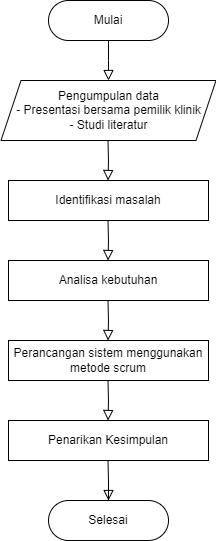
\includegraphics[width=4cm]{gambar/tahapan penelitian fix.png}
	\caption{Tahapan penelitian} 
	\label{Gambar:usecaseadminjurnalpertama}
\end{figure}

\section{Pengumpulan Data}

Peneliti mengambil data dari presentasi bersama dengan pemilik klinik \emph{moist care} dan klien dari penelitian ini yaitu ibu Irma Puspita Arisanti. Untuk dokumentasi foto pada saat presentasi dapat dilihat pada Lampiran A. Peneliti juga melakukan studi literatur dengan membaca jurnal-jurnal yang berkaitan dengan topik penelitian serupa. 

\section{Analisa Kebutuhan}
Berikut merupakan perangkat keras dan perangkat lunak yang penulis butuhkan dalam merancang sistem informasi keperawatan luka:

Perangkat keras berupa:
\begin{enumerate}
	
\item Laptop dengan spesifikasi Processor Intel Core i5 generasi ke-3 dan RAM 12 GB.
	
\end{enumerate}

Perangkat lunak berupa:
\begin{enumerate}
\item Windows 10 \emph{Operating System}.

\item Figma sebagai alat untuk mendesain tampilan UI/UX.

\item \emph{Visual Studio Code} untuk pembuatan sistem informasi keperawatan luka.

\item \emph{Python} sebagai bahasa pemrograman yang peneliti gunakan.

\item \emph{Flask} sebagai web framework yang akan digunakan.

\item MongoDB sebagai basis data
\end{enumerate}

\section{Perancangan Sistem Menggunakan \emph{Scrum}}

\emph{Website} aplikasi yang dibuat dalam penelitian ini dikembangkan dengan menggunakan metode \emph{scrum}. Penjelasan rinci tentang metode \emph{scrum} akan disajikan pada sub bab di bawah ini.

\subsection{\emph{Product Backlog}}

Tahap \emph{Product backlog} ini berfungsi untuk menterjemahkan seluruh fitur yang akan diimplementasikan pada aplikasi. Rincian \emph{Product Backlog} yang akan diimplementasikan pada \emph{website} aplikasi dapat dilihat pada tabel di bawah ini.

\begin{table}[H]
	\centering
	\caption{\emph{Product Backlog}}
	\label{tabel_input}
	\begin{tabular}{|c|l|c|c|}
		\hline
		\textbf{No} & \textbf{\emph{User Story}} & \textbf{\emph{Priority}} & \textbf{\emph{Sprint} No.} \\
		\hline
		
		1 & 
		Pembuatan akun pasien & \emph{High}
		& 1 \& 2 \\
		\hline
		
		2 & 
		Dashboard klinik  & \emph{High}
		& 1 \& 2 \\
		\hline
		
		3 & 
		Pemeriksaan kesehatan & \emph{High}
		& 1 \& 3 \\
		\hline
		
		4 & 
		Proses pengobatan luka & \emph{High}
		& 1 \& 3 \\
		\hline
		
		5 & 
		Pendaftaran pasien berobat & \emph{High}
		& 1 \& 3 \\
		\hline
		
		6 & 
		Pengelolaan antrian & \emph{High}
		& 1 \& 4 \\
		\hline
		
		7 & 
		Administrasi keuangan  & \emph{High}
		& 1 \& 4 \\
		\hline
		
	\end{tabular}
\end{table}

\emph{Product backlog} yang dibuat memiliki 4 kolom yang di antaranya adalah sebagai berikut:

\begin{enumerate}
	\item \emph{User Story}
	
	Kolom \emph{user story} berisi fitur-fitur yang akan dibuat pada aplikasi.
	
	\item \emph{Priority}
	
	Kolom \emph{priority} berisi tingkat priortas dari \emph{user story}, dimana prioritas \emph{high} merupakan fitur yang mempunyai peran penting pada penelitian ini.
	
	\item \emph{Sprint} No.
	
	Kolom \emph{sprint} no. berisi informasi tentang urutan pengerjaan fitur \emph{sprint} tersebut akan dibuat.
\end{enumerate}

\subsection{\emph{Sprint Backlog}}
Sebelum \emph{sprint} dimulai dilakukan \emph{sprint backlog}, \emph{sprint backlog} berisikan daftar pekerjaan yang keputusannya diambil dari \emph{product backlog}. Dengan adanya \emph{sprint backlog} semua anggota tim bisa melihat perkembangan dari setiap pekerjaan. Pada penelitian peneliti menggunakan tiga status perkembangan yaitu harus dikerjakan, sedang dikerjakan, selesai, next \emph{sprint} dan tidak selesais.

\subsection{\emph{Sprint}}
Setelah perencanaan \emph{sprint backlog} sudah dibuat, maka pengerjaan \emph{sprint} sudah bisa dimulai dan mengikuti jadwal pengerjaan yang telah disepakati bersama tim. Interval \emph{sprint} yang digunakan adalah dua minggu.

\subsection{\emph{Deploy}}
Setelah semua pekerjaan \emph{sprint} yang telah direncanakan pada sprint backlog selesai maka aplikasi akan di \emph{deploy}.

\begin{comment}
	
	Mockup administrasi keuangan
	Penjelasan UI/UX bab 2 revisi banyak
	API route setiap fitur
	
	
	menjelaskan sistem utuh yang dibuat salsa
	membuat product backlog yang berisi 3 sprint, rancangan ui dan data base
	
	sprint 1 berisi
	1. database diagram
	2. produk backlog
	3. rancangan ui/ux
	yang dibagi per iterasi
	
	implementasi sprint 1
	
	acc sps

\begin{table}[H]
	\centering
	\caption{\emph{Sprint}-2 \emph{Backlog}}
	\label{tabel_input}
	\begin{tabular}{|c|m{6 cm}|m{6 cm}|}
		\hline
		\textbf{No} & \textbf{\emph{User Story}} & \textbf{\emph{Task}}\\
		\hline
		
		1 & 
		Pembuatan akun pasien & 1.Pembuatan akun pasien.\\
		
		& 
		& 2.Menerima pendaftaran akun pasien baru\\
		\hline
		
		2 & 
		Pendaftaran pasien berobat & 1.Melakukan pendaftaran pasien yang berobat pada hari H.\\
		
		& 
		& 2.Mencari data pasien berdasarkan \emph{Medical} ID/Nomor BPJD/NIK.\\
		
		& 
		& 3.Sistem mampu mengeluarkan nomor antrean pengobatan secara \emph{real time}.\\
		\hline
		
	\end{tabular}
\end{table}

\begin{table}[H]
	\centering
	\caption{\emph{Sprint}-3 \emph{Backlog}}
	\label{tabel_input}
	\begin{tabular}{|c|m{5 cm}|m{6 cm}|m{1 cm}|}
		\hline
		\textbf{No} & \textbf{\emph{User Story}} & \textbf{\emph{Task}} & \textbf{\emph{Status}} \\
		\hline
		
		1 & 
		Pengelolaan antrean & 1.Menentukan kuota jumlah pelayanan pasien pada hari pelayanan
		& belum selesai \\
		
		& 
		& 2.Menentukan kuota pelayanan pasien \emph{online} pada hari pelayanan.
		& \\
		
		& 
		& 3.Menentukan kuota pelayanan pasien \emph{offline} pada hari pelayanan.
		& \\
		\hline
		
		2 & 
		Proses pengobatan & 1.Melihat hasil pengkajian luka dengan mencari berdasarkan NIK/Nama
		& belum selesai \\
		
		& 
		& 2.Melihat \emph{database} foto luka yang dikategorikan berdasarkan perawat
		& \\
		
		& 
		& 3.Inventarisasi komponen kesehatan yang masuk ke dalam klinik beserta harganya sebagai \emph{base cost}.
		& \\
		
		& 
		& 4.Menentukan tarif pengobatan diluar obat dan balutan(biaya layanan, dll).
		& \\
		\hline
		
	\end{tabular}
\end{table}

\begin{table}[H]
	\centering
	\caption{\emph{Sprint}-4 \emph{Backlog}}
	\label{tabel_input}
	\begin{tabular}{|c|m{5 cm}|m{6 cm}|m{1 cm}|}
		\hline
		\textbf{No} & \textbf{\emph{User Story}} & \textbf{\emph{Task}} & \textbf{\emph{Status}} \\
		\hline
		
		1 & 
		Administrasi keuangan & 1.Verifikasi dan validasi biaya tagihan
		& belum selesai \\
		\hline
		
		2 & 
		Dashboard klinik & 1.Melihat statistik kinerja perawat per bulan
		& belum selesai \\
		
		& 
		& 2.Melihat \emph{cost} dari inventarisasi yang tersedia dan aset yang masih berjalan.
		& \\
		
		& 
		& 3.Melihat besar \emph{cost} perawatan pasien.
		& \\
		
		& 
		& 4.Melihat \emph{income} masuk klinik
		& \\
		
		& 
		& 5. Melihat \emph{balance} keuangan dalam satu bulan
		& \\
		\hline
		
	\end{tabular}
\end{table}

\end{comment}

%-----------------------------------------------------------------
%Disini akhir masukan Bab
%-----------------------------------------------------------------


%-----------------------------------------------------------------
% Disini awal masukan untuk Daftar Pustaka
% - Daftar pustaka diambil dari file .bib yang ada pada folder ini
%   juga.
% - Untuk memudahkan dalam memanajemen dan menggenerate file .bib
%   gunakan reference manager seperti Mendeley, Zotero, EndNote,
%   dll.
%-----------------------------------------------------------------

\bibliography{daftar-pustaka}
\bibliographystyle{apa}
\addcontentsline{toc}{chapter}{DAFTAR PUSTAKA}
%-----------------------------------------------------------------
%Disini akhir masukan Daftar Pustaka
%-----------------------------------------------------------------


\end{document}